\chapter{Sensitivity of the SuperNEMO demonstrator to the $\zeronu$}
\label{ch:sensitivity}

In this chapter, we present a study aiming to evaluate the SuperNEMO's sensitivity to the $\zeronu$ decay, and the corresponding effective neutrino mass.
Studies of this kind have already been conducted, and the final detector, based on the NEMO-$3$ technology, is expected to exclude half-lives up to $1.2\times 10^{26}$ y ($90\%$ CL), with an exposure of $500$ kg.y for the \Se\footnote{Supposing the  $\zeronu$ decay of \Se\ occurs through the exchange of a light Majorana neutrino.}~\cite{art:SuperNEMO2010}.
In order to assess the feasibility of such a large-scale detector, the SuperNEMO demonstrator started to be installed in early $2015$, at the Laboratoire Souterrain de Modane.
With an exposure of $17.5$ kg.y, this demonstrator could reach a sensitivity on the $\zeronu$ process of \Se\ $5.3\times 10^{24}$ y ($90\%$ CL) \cite{CalvezThesis}.

A copper coil was designed to deliver a uniform $25$~Gauss magnetic field inside the wire chamber, to bend the charged particles trajectories, thus making it possible to discriminate between electrons and positrons.
However, studies lead by the collaboration determined that this field could be impacted by the detector material (especially by the calorimeter magnetic shields), leading to strong variations in intensity and a loss of energy resolution~\cite{CalvezThesis}\cite{internal:magnetic_field}.
We aim to explore the impact, on both the demonstrator and final detector sensitivity, of the presence of this magnetic field.
The findings of this study will participate in the final decision on the installation of the coil.
In a context of investigating the demonstrator and final detector's capabilities, different internal source contamination levels are considered.
The topology of interest is the two electrons topology, and we use the total energy sum to discriminate the signal from the background events.
Thanks to SuperNEMO tracking capabilities, topological informations are exploited to improve the sensitivity.
To go further, we also explore the possibility of studying the $\zeronu$ decay of other $\beta\beta$ isotopes.

\section{The $\zeronu$ signal and background model}
\label{sec:sensitivity_simus}

A full simulation for the demonstrator was performed, in order to determine the upper limit on $\zeronu$ half-life that can be probed with SuperNEMO.
This sensitivity depends on the number of selected background events.

Due to the time it would take to simulate every expected background contribution, the choice of a simplified model, containing only the most harmful backgrounds to the $\zeronu$ decay search, was adopted.
These backgrounds are the $\twonu$ decay, contaminations of the source in \Tl\ and \Bi, and contamination of the tracker gas with Radon.
The number of natural isotope decay events expected depends on their activities inside the source foils (for \Tl\ and \Bi), or on the tracker's wires (for \Rn\ decaying in \Bi).
It was necessary, during the design of the detector, to constrain the maximal tolerable activities, to guarantee a high sensitivity to the $\zeronu$ disintegration~\cite{internal:SNphysicsCase}.
The collaboration then established recommendations for maximum levels of internal background, expressed in number of disintegrations per second, for a unit mass of $\beta\beta$ isotope, or for a unit volume of gas.
These are the so-called specified activities.
The amount of expected double $\beta$ decays is driven by its half-life value: the higher the half-life, the lower its contribution in the total number of expected background.
For \Se\ sources, we take the $\twonu$ half-life measured by NEMO-$3$, $\Ttwonu~=~9.39~\pm~0.17$~(stat)~$\pm~0.58$~(syst)~$\times~10^{19}$~years~\cite{art:NEMO2018}.
Moreover, we choose to consider the best limit set on the $\zeronu$ process, of $\Tbeta > 2.5\times 10^{23}$~y~\cite{art:NEMO2018}.
This value is given for illustration purposes only and is not used to estimate the sensitivity of the detector.
In the Tab.~\ref{tab:sensitivity_simulations} is summarised the expected number of signal and background events, per disintegration unit per second, for one kg of source material, or for one m$^{3}$ of gas inside the tracker.
\begin{table}[h]
  \centering
  \begin{tabular}{|l|cc|c|}
    \hline
    Process &\multicolumn{2}{c|}{Expected decays} & Simulated decays \\
    & Demonstrator & Final detector & \\
    \hline\hline
    $\zeronu$ ($\Tbeta = 2.5\times 10^{23}$ y) & $3.6\times 10^{2}$ & $1.0\times 10^{4}$ & $1.0\times 10^{7}$ \\
    $\twonu$ ($\Ttwonu = 9.39\times 10^{19}$ y) & $9.5\times 10^{5}$ & $2.7\times 10^{7}$ & $1.0\times 10^{7}$ \\
    \Tl\ ($\mathcal{A}^{\text{Tl}} = 2~\mu$Bq/kg)  & $1.1\times 10^{3}$ & $3.1\times 10^{4}$ & $1.0\times 10^{7}$ \\
    \Bi\ ($\mathcal{A}^{\text{Bi}} = 10~\mu$Bq/kg) & $5.5\times 10^{3}$ & $1.6\times 10^{5}$ & $1.0\times 10^{7}$ \\
    \Rn\ ($\mathcal{A}^{\text{Rn}} = 0.15$ mBq/m$^{3}$) & $1.8\times 10^{5}$ & $7.2\times 10^{6}$ & $1.0\times 10^{8}$ \\
    \hline
  \end{tabular}
  \caption{Expected and simulated decays for different processes, both for the demonstrator ($17.5$ kg.y) and for the final detector exposures ($500$ kg.y), assuming target background activities are reached: $\mathcal{A}^{\text{Tl}}~=~10\,\mu$Bq/kg, $\mathcal{A}^{\text{Bi}}~=~2\,\mu$Bq/kg, $\mathcal{A}^{\text{Rn}}~=~0.15$ mBq/m$^{3}$.
    The measured half-life $\Ttwonu~=~9.39\times~10^{19}$ y for \Se's $\twonu$ is taken, and we assume $\Tbeta = 2.5\times 10^{23}$ y~\cite{art:NEMO2018}.
    \label{tab:sensitivity_simulations}}
\end{table}
These figures are presented both for the SuperNEMO demonstrator and final detector.
They represent the total number of disintegrations, without taking into account any technique to reject background, and for the total energy window.
Nevertheless, the number of decays presented in this table are expected to be extremely reduced, notably by the application of event selections aimed at maximising the sensitivity to the excluded $\zeronu$ half-life (Sec.~\ref{sec:sensitivity_ev_selection}).
This effect is augmented by the fact that, for the current sensitivity analysis, we focus on a narrow energy window, called \emph{region of interest}, whose usefulness is described in detail in Sec.~\ref{sec:sensitivity_ev_selection}.
Therefore, to properly conduct this sensitivity study, it was necessary to simulate a large number of events, so that the signal and backgrounds are correctly represented in the region of interest.
In the table are presented the total amount of simulated events for each process.

%% c'est pas plutôt à cause du fait que tous les decays de ces isotopes ne sont pas intéressants ?
%% du coup dans la topologie 2e il ne reste plus rien

\subsection{The $\zeronu$ signal}

The SuperNEMO detector was designed to search for the never-observed $\zeronu$ decay.
In the following, we assume the underlying mechanism for this decay is the exchange of a light Majorana neutrino, the so-called mass mechanism (MM), as it is the most widespread mechanism.
The hypothetical $\zeronu$ signal would be detected as an excess of events in the region of interest, with respect to the predicted background contamination levels.
Some $10^{7}$ $\zeronu$ events were simulated inside the source foils, using the DECAY$0$ software~\cite{art:decay0}.

\subsection{Inside detector backgrounds}

In addition with the $\zeronu$ decay, we simulated different types of backgrounds, that could mimic the searched signal.

\subsubsection{Internal backgrounds}

The so-called \emph{internal backgrounds} stand for decays occurring inside the source foils, presenting the same signature as the $\zeronu$ signal.
These backgrounds, already introduced earlier, are the $\twonu$ of the source isotope, as well as disintegrations of \Tl\ and \Bi\ inside the source foils.

\subsubsection*{The $\twonu$ process}

In the full energy range, the allowed $\twonu$ decay stands as the dominant internal background type.
The corresponding two-electrons energy sum spectrum is a continuum, whose ending point should stands at $\Qbb = 2.99$~MeV, but is slightly shifted by the detector's energy resolution.
We simulated $10^{7}$ events of this decay inside the source foils, in the full energy window.
However, above a certain energy value, the number of $\twonu$ events decreases very quickly.
To offset this effect, we simulated additional $10^{7}$ of this decay on a slightly reduced energy range, that is to say above $2$~MeV.
The second set of simulations is normalised with the first one.
In this way, the lack of $\twonu$ simulated events in the high-energy tail is avoided, without requiring too high computational resources.

\subsubsection*{Source foils contamination by natural isotopes}

As described in Sec.~\ref{subsec:SNbkg_internal}, after sources purification, remaining natural isotopes such as \Tl\ or \Bi\ can still be present inside the foils, constituting the principal internal source of background, with the $\twonu$ decay.
We simulated $10^{7}$ decays both for the two isotopes, inside the source foils.

\subsubsection{Tracker contamination by natural isotopes}

The presence of gaseous \Rn\ inside the tracker, mainly deposited on the copper wires, can produce events similar to internal ones.
In fact, one of the progeny of \Rn, the \Bi, can decay on (or near) a foil, and appear with a two-electron ($2e$) topology, becoming hard to distinguish from a double beta decay candidate.
As this isotope is distributed throughout the whole tracking detection volume, to study the experiment's sensitivity, we simulated a large quantity of this decay, that is to say $10^8$ decays on the tracker wires.
%This way, we maximise the amount of \Bi\ events, coming from \Rn\ decays, in the region of interest.


\subsection{External backgrounds}
\label{subsec:ext_bkg}

This background category is populated by the external $\gamma$-ray flux produced by radioactive isotope decays (mostly \K, \Bi\ and \Tl) in detector components or surrounding laboratory rocks, as well as neutron interactions in the external iron shield.
As external background simulations would be very consuming in terms of computing ressources, it is important to ensure that they are necessary.
The NEMO-$3$ experiment set a limit on the external background number of counts, of $<0.2$ events in the $2e$ topology, for the energy range [$2.8$;$3.2$]~MeV (two electrons energy sum), for an exposure of $34.3$ kg·y, with $^{100}$Mo sources~\cite{art:NEMO2015}.
Radiopurity measurements of the SuperNEMO PMTs allow to conclude that the total \Bi\ activity is $35\%$ lower than for those of NEMO-$3$~\cite{docdb:perrot2017}, which is encouraging.
Unfortunately, these measurements also revealed that the total budget in \Tl\ isotope is $150\%$ higher than NEMO-$3$.
This could lead us to think that the external background contribution for SuperNEMO could be higher than that of NEMO-$3$.
However, on that level, the most notorious difference between the two detectors is the fact that the SuperNEMO scintillator blocks are thicker than those of NEMO-$3$.
Therefore, a gamma is more likely to be detected before crossing the source foils and, in that case, the event would not contribute to the background in the $2e$ channel.
Even if the regions of interest are slightly different between these two experiments, it produces negligible increase on the external background contribution\footnote{A study conducted by the SuperNEMO collaboration shown that only $0.73$ additional external background events would have been expected for the NEMO-$3$ detector, if instead of taking the [$2.8$;$3.2$]~MeV energy range, we would have considered the [$2.7$;$3.15$]~MeV region of interest.}.
After all, given the fact that SuperNEMO is expected to be better than NEMO-$3$ at rejecting external background events, we consider that all external backgrounds from outside the foil, apart from \Rn\ in the tracking volume, are expected to be negligible, and were not simulated.


\section{Event selection}
\label{sec:sensitivity_ev_selection}

For SuperNEMO, the $\zeronu$ signature is two-electrons events, emitted simultaneously from the same vertex on the source foils, with an energy sum compatible with $\Qbb = 2.99$~MeV for the \Se.
Therefore, we conducted this analysis selecting only events matching the $2e$ topology, where a reconstructed particle is tagged as an electron if it has
\begin{itemize}
\item a vertex on the source foils,
\item a reconstructed track inside the wire chamber,
\item an associated calorimeter hit,
\item and a final criterion depending on the case under consideration.
  In fact, as announced, this study also aims at considering two separate magnetic field cases.
  One where the magnetic field is aligned with the $Z$ (vertical) axis of the detector, and has a uniform value of $25$ Gauss, and one where the field is turned off.
  In the first case, particles such as electrons and positrons of a few~MeV have a curved trajectory in the tracker.
  In the second case, the tracks of the particles may be similar to straight lines (not to mention the possible multiple scattering on the wires of the tracker).
  It is then necessary to adapt the selection of events to each case.
  We then consider an additional criterion: a particle is identified as an electron if its track has a negative curvature.
  In the following, we present results where the magnetic field is turned on.
  The off-field study is addressed in Sec.~\ref{sec:magnetic_field}.
\end{itemize}
All these selections represent the so-called \emph{first-order} cut-offs.
We present the total energy spectra for each simulated process, after application of these cut-offs, in Fig.~\ref{fig:energy_spectra}.
\begin{figure}[h]
\centering
\begin{subfigure}[t]{0.7\textwidth}
  \centering
  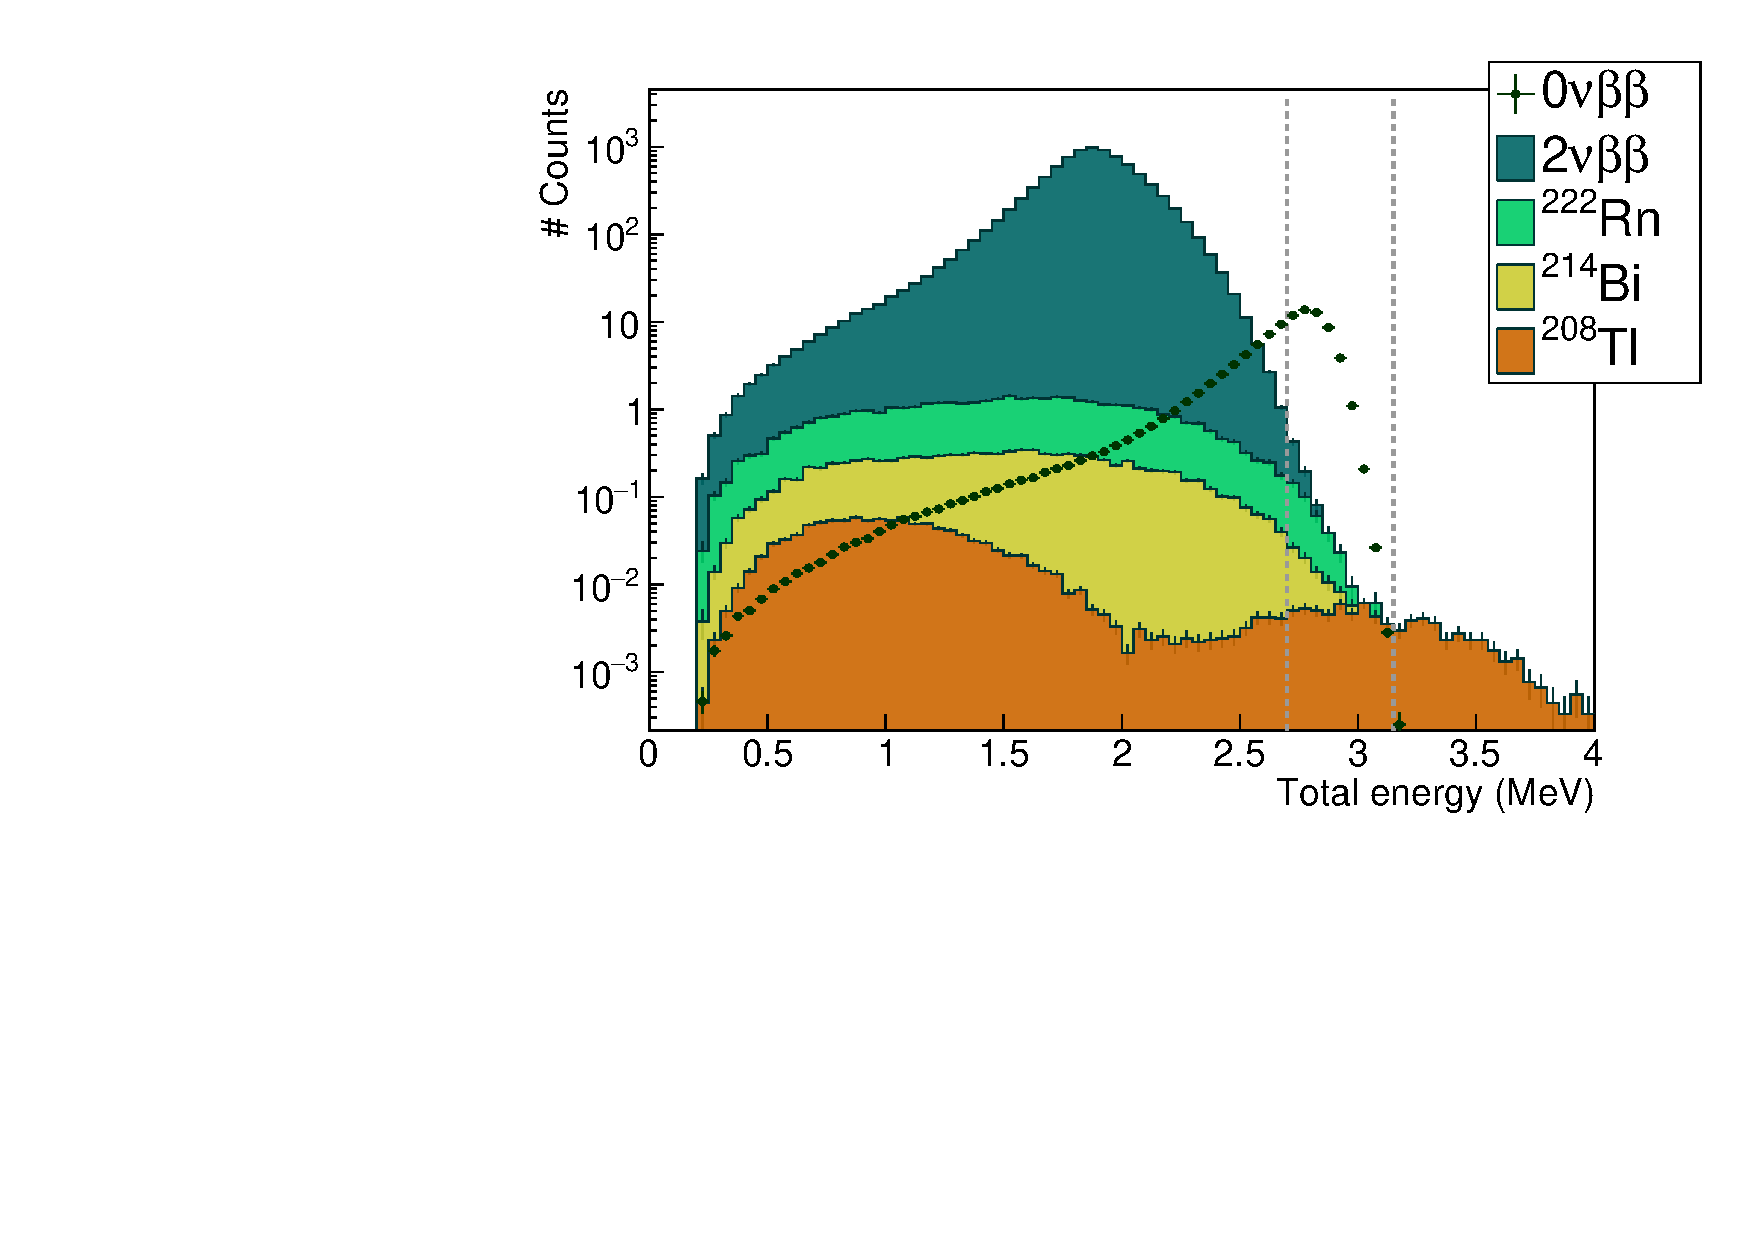
\includegraphics[width=1.1\textwidth]{Sensitivity/fig_sensitivity/energy_spectrum_with_B_82Se.pdf}
  \captionsetup{justification=centering}
  \caption{
    \label{subfig:energy_spectra_full}}
\end{subfigure}
\hfill
\begin{subfigure}[t]{0.7\textwidth}
  \centering
  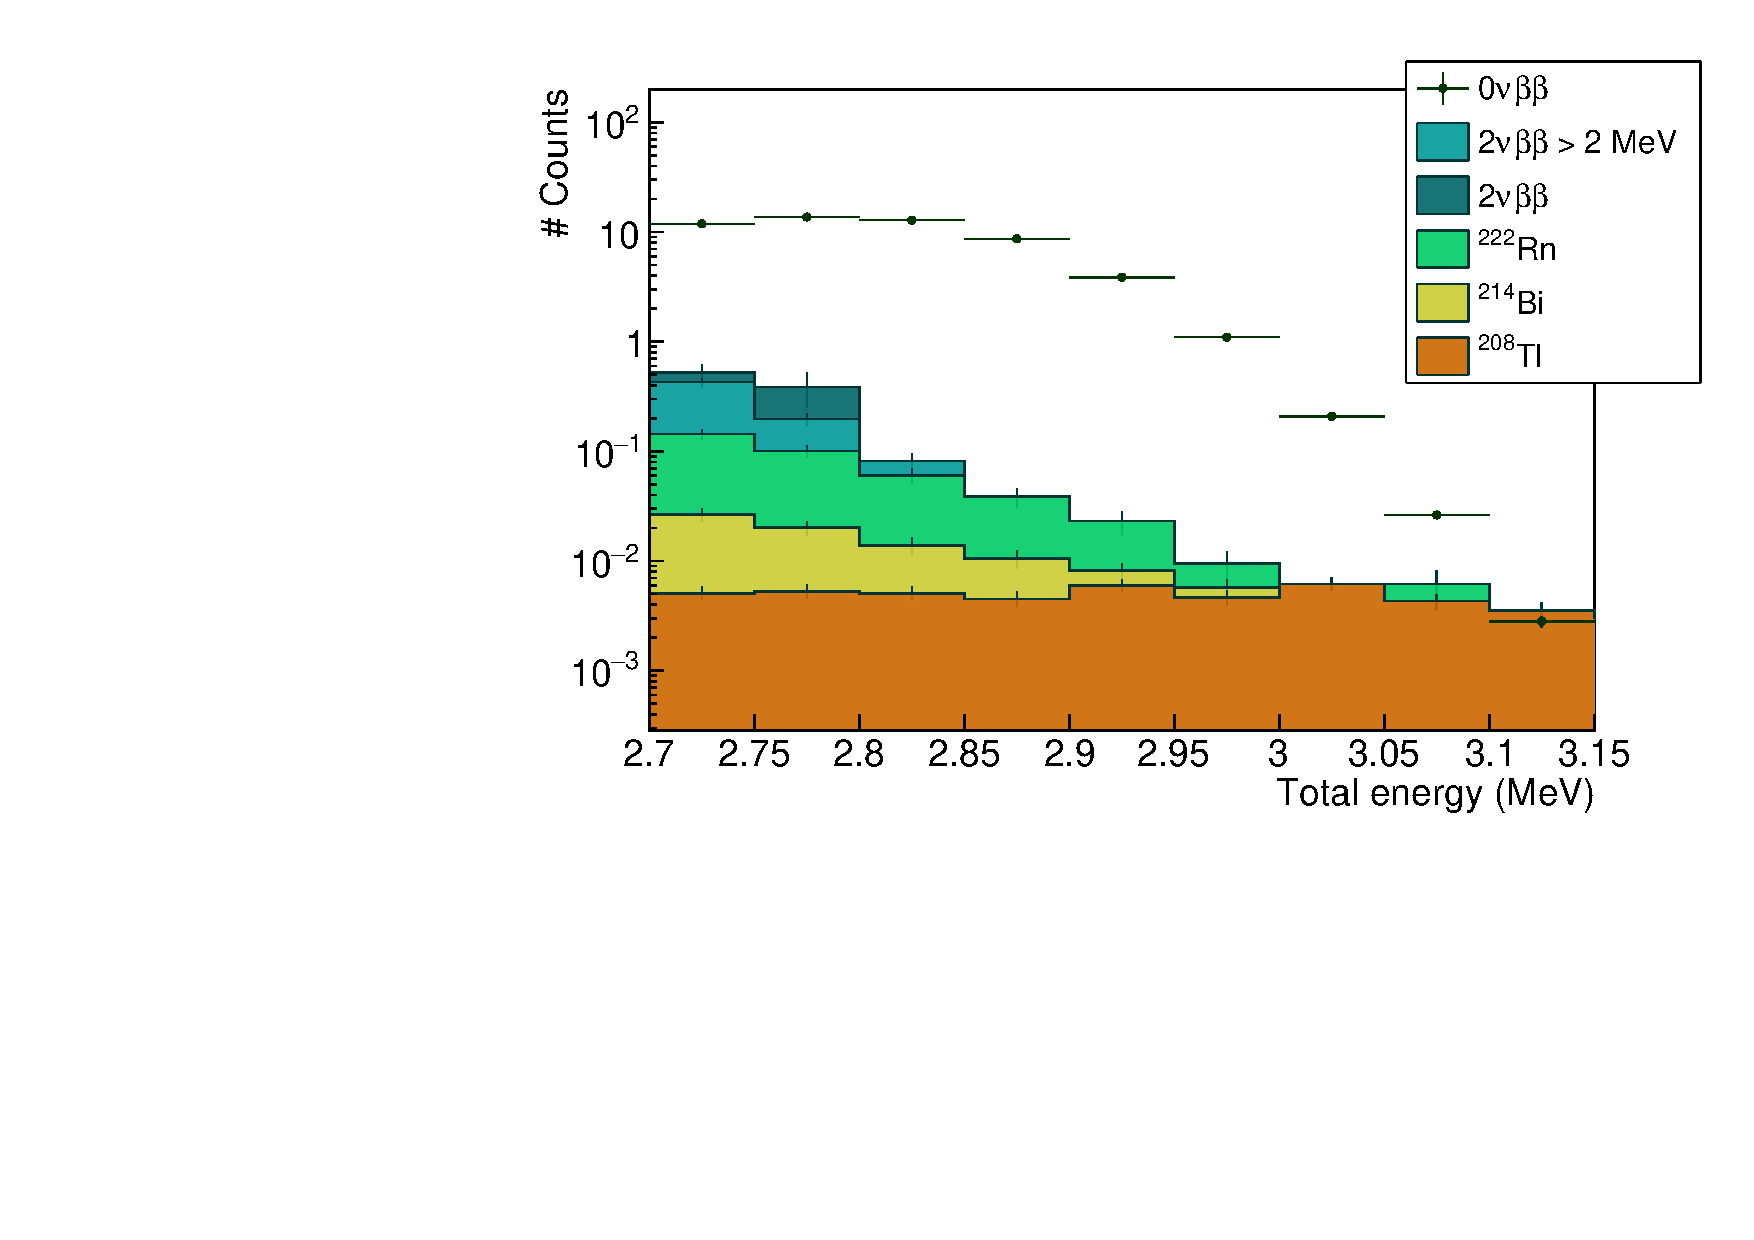
\includegraphics[width=1.1\textwidth]{Sensitivity/fig_sensitivity/energy_spectrum_with_B_82Se_zoom.pdf}
  \captionsetup{justification=centering}
  \caption{
    \label{subfig:energy_spectra_zoom}}
\end{subfigure}
\caption{Total energy spectra for the $\zeronu$ signal and main backgrounds, for (a) the full energy range, and (b) for the [$2.7$;$3.15$]~MeV energy range, whose optimisation is discussed in Sec.~\ref{sec:Nbkg_ROI}.
  \label{fig:energy_spectra}}
\end{figure}
We present results for the specific case were of the demonstrator (\Se\ sources, $17.5$~kg.y exposure), with the specified internal contamination levels ($\mathcal{A}^{\text{Tl}} = 2\,\mu$Bq/kg and $\mathcal{A}^{\text{Bi}} = 10\,\mu$Bq/kg).

If the $\zeronu$ decay is detected, its energy distribution would be a peak, located at the end-point of the $\twonu$ energy distribution, that is to say at the total available energy, $\Qbb = 2.99$~MeV.
In principle, this peak is infinitly thin, as the two electrons of this decay would share the total available energy.
However, the two emitted electrons may lose some of their energy in the detector, mainly inside the dense source material and the wire chamber, which would lead to the widening of this peak.
It is also expected to be shifted towards small energies, by the calorimeter energy resolution and the straggling of energy losses in the detector.
All this is at the origin of the asymmetrical energy distribution shown in the figure.
Concerning the $\twonu$ energy spectrum, we present the events simulated in the total energy range, in addition with the $\twonu$ simulations with an energy $>~2$~MeV.
At the end, the two sets of simulation are normalised.
% The progeny of \Rn\ produces $\gamma$-rays and $\beta$ decays accompanied by internal conversion (IC), Møller or Compton scattering, the dominant mechanism being the first one.
Whatever their origin, either \Rn\ contaminations inside the tracker gas, or internal contaminations of the source foils, the two \Bi\ energy distributions have nearly the same shapes.
%%Therefore, given the activities of \Rn\ in the tracker and \Bi\ inside the source foils, theses two background types both contribute at the same level in the full energy range.
The \Tl\ spectrum reveals the internal conversion of the $2.614$~MeV gamma, emitted after \Tl\ $\beta^{-}$ disintegrations.
All spectra are normalised to the natural isotopes specified activities, and the half-lifes values.

A widespread technique consists in constraining the $\zeronu$ decay searches to a narrow energy range, the so-called \emph{region of interest} (ROI), materialised by the two vertical dashed lines in the figure.
In the following, we expose general principles leading to the determination of the best limit on $\Tbeta$, in the appropriate region of interest.
We illustrate the reasoning with the demonstrator, specified activities, on-magnetic field case.
However, the technique presented remain valid for all exposures, internal contamination levels and field conditions.
The impact of all these parameters is detailed in the rest of this chapter.
%The optimisation of this energy window consists of cutting the full energy range in several sub-ranges, and compute the selection efficiencies for all energy sub-ranges.

\section{Demonstrator sensitivity to the $\zeronu$ decay of \Se}
\label{sec:Nbkg_ROI}

The SuperNEMO demonstrator is designed to measure $\beta\beta$ decays of radiaoctive emiters.
In case a the non-obervation of this process, the demonstrator would set an upper-limit on the half-life $\Tbeta$, and on the effective neutrino mass $\mbb$.

\subsection{Sensitivity to the $\zeronu$ half-life}

In case of the non-observation of a $\zeronu$ signal, the expected upper limit on the half-life is provided for a given [$E_{\text{min}}$;$E_{\text{max}}$] energy range, and depends on the characteristics of the detector.
First, it depends on the signal detection efficiency, $\epsilon_{0\nu}$, in this energy window, secondly on the source isotope nature, as well as the detector's exposure $m\times t$.
It follows
\begin{equation}
  \Tbeta > \frac{\mathcal{N}_{\text{A}}\ln{2}}{M}\times \frac{\epsilon_{0\nu}\times m\times t}{N_{0\nu}^{\text{excl.}}}\,,
  \label{eq:tbeta_limit}
\end{equation}
with $\mathcal{N}_{\text{A}}$ the Avogadro number, $m$ the quantity of isotope in the source foils, $M$ its molar mass, and $t$ the total time of data acquisition.
$N_{0\nu}^{\text{excl.}}$ is the number of signal events excluded, calculated with the Feldman-Cousins statistics from the total expected number of background events.
The Feldman-Cousins statistics~\cite{art:feld-cous} is a wide-used method in rare events search experiments, providing confidence intervals for upper limits in the case of Poisson processes with background.
We use this method in the framework of this analysis to provide a limit, at $90\%$ CL, on the number of excluded signal events $N_{0\nu}^{\text{excl.}}$, on the basis of the expected number of background events, given below.
\begin{itemize}
\item The $\twonu$ background\\
  In Eq.~\eqref{eq:tbeta_limit}, we defined the upper limit on $\Tbeta$ from the number of excluded signal events, and the signal selection efficiency $\epsilon_{0\nu}$.
  In a similar manner, we can define the number of expected $\twonu$ events, $N_{2\nu}$, from the half-life $\Ttwonu$ and the $\twonu$ selection efficiency, $\epsilon_{2\nu}$, as
  \begin{equation}
    N_{2\nu} = \frac{\mathcal{N}_{\text{A}}\ln{2}}{M}\times\frac{\epsilon_{2\nu}\times m\times t}{\Ttwonu}\,.
    \label{eq:N_2nu}
  \end{equation}
\item Natural radioactive backgrounds\\
  We consider the background massic activities $A_{\text{rad.}}$, and $\epsilon_{\text{rad.}}$ their selection efficiencies in a given energy window.
  The number of background events is therefore given, for the \Tl\ and \Bi\ internal contaminations, as
  \begin{equation}
    N_{\text{rad.}} = A_{\text{rad.}}\epsilon_{\text{rad.}}\times m\times t\,,
  \end{equation}
  where $A_{\text{rad.}}$ is given in Bq/kg.
  Similarly, for the \Rn\ background,
  \begin{equation}
    N_{\text{rad.}} = A_{\text{rad.}}\epsilon_{\text{rad.}}\times V\times t\,,
    \label{eq:N_Rn}
  \end{equation}
  with $V = 15.3$ m$^{3}$ the tracker volume, and where $A_{\text{rad.}}$ represents here a volumic activity, given in Bq/m$^{3}$.
\end{itemize}
All these equations, similarly as Eq.~\eqref{eq:tbeta_limit}, are valid for a given energy range [$E_{\text{min}}$;$E_{\text{max}}$].
To find the optimal energy interval for the search of the $\zeronu$ decay, that is to say the one maximising the limit on $\Tbeta$, we must vary the E$_{\text{min}}$ and E$_{\text{max}}$ bounds.

As can be seen in Fig.~\ref{fig:energy_spectra}, beyond $3$~MeV, the number of background events becomes negligible compared with the $\zeronu$ decay.
Indeed, the \Tl\ background dominates at these energies, where it does not exceed one count for E$>3.2$~MeV.
This is why the upper limit E$_{\text{max}}$ of the energy interval has only a limited impact on the search for the best ROI.
It is then natural to study mainly the influence of the lower limit E$_{\text{min}}$.
Therefore, the selection efficiencies, entering in the calculation of the $\Tbeta$ upper limit, are presented in Fig.~\ref{fig:efficiency_spectra}, as a function of $\text{E}>\text{E}_{\text{min}}$.
\begin{figure}[h]
  \centering
  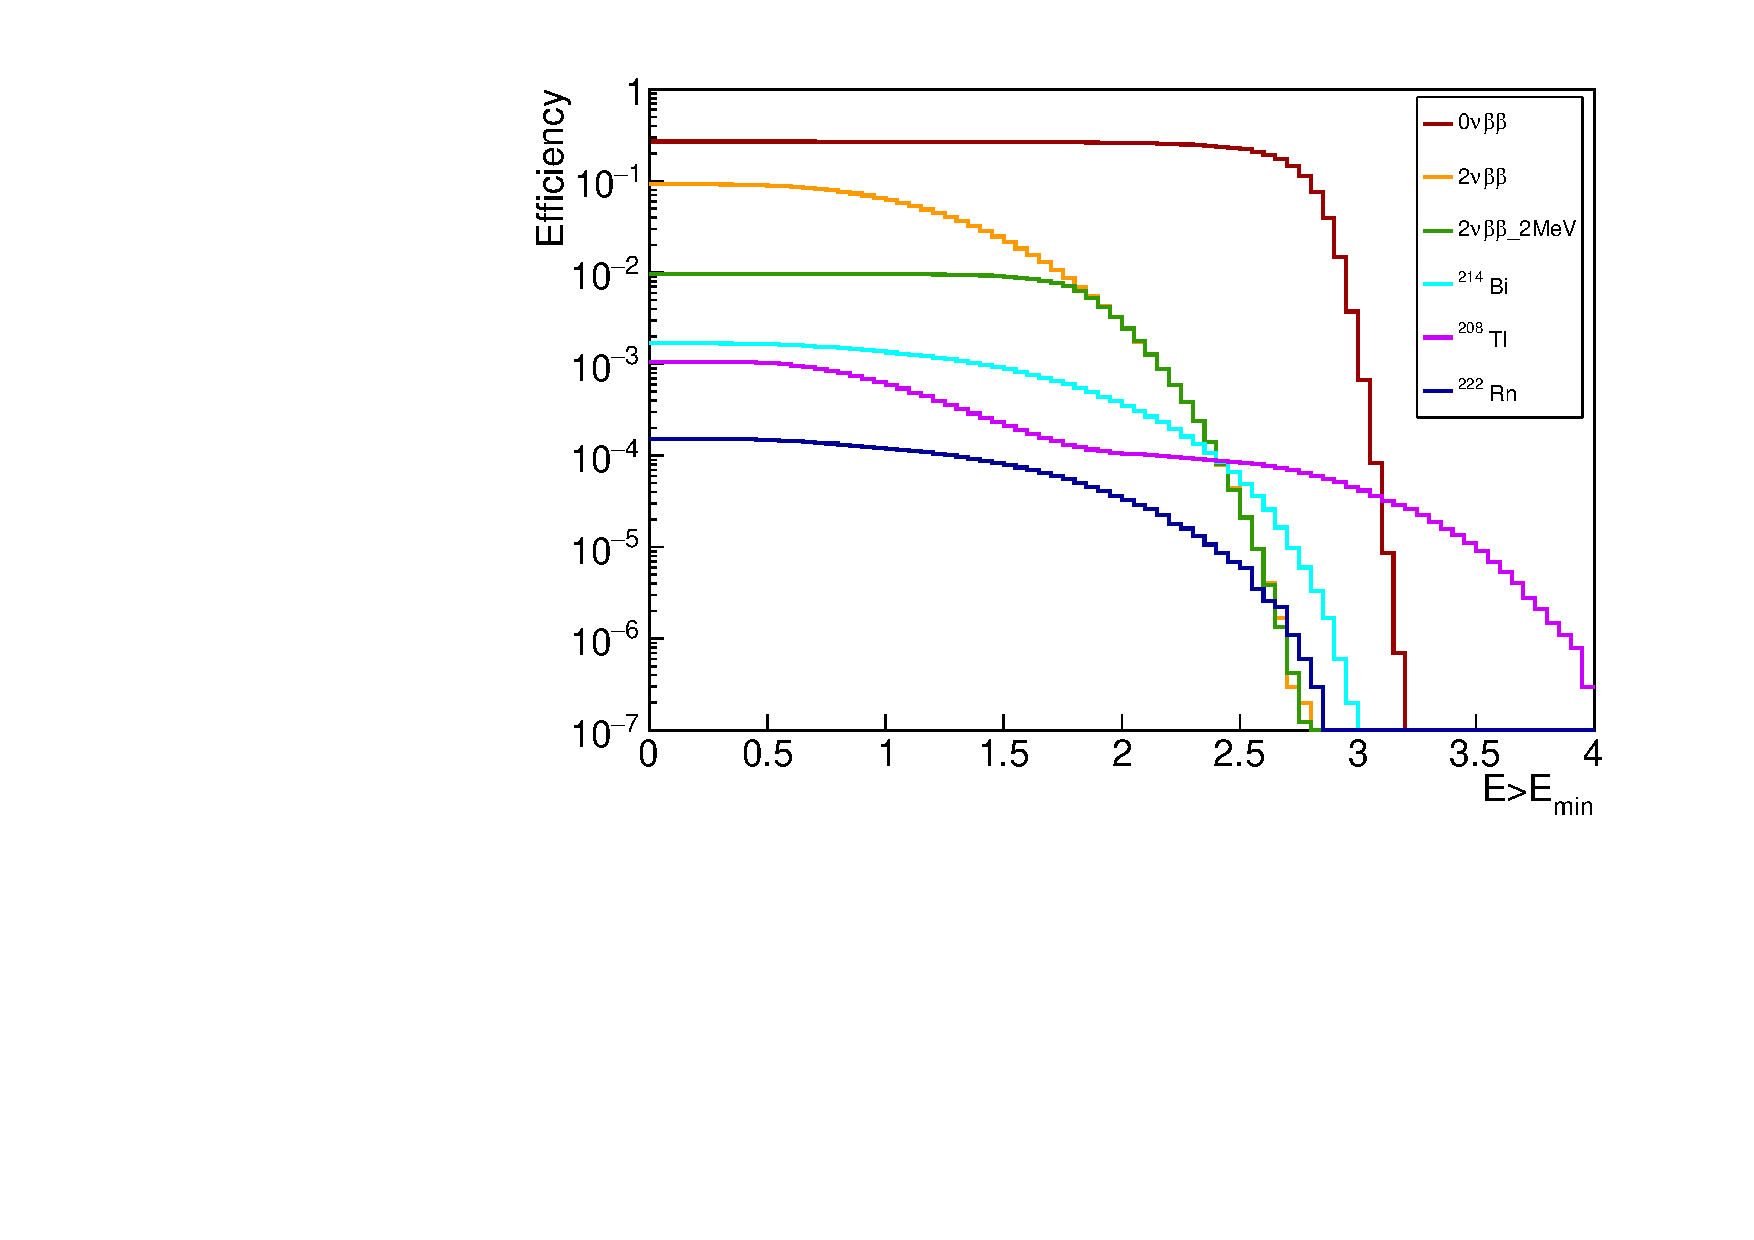
\includegraphics[width=0.8\textwidth]{Sensitivity/fig_sensitivity/efficiency_spectrum_with_B_82Se.pdf}
  \caption{Efficiency spectra as a function of $\text{E}>\text{E}_{\text{min}}$, for the $\zeronu$ signal (dashed black line) and for the main backgrounds (plain lines).
    The two vertical grey lines represent the final ROI optimised for the case of the demonstrator, taken the specified isotope activities.
    \label{fig:efficiency_spectra}}
\end{figure}
We remind a selection efficiency $\epsilon$ is the ratio of the number of selected events, to the number of simulated events.
As a matter of fact, we look for an energy region where $\epsilon_{0\nu}$ is high, and where selection efficiencies for the background are low.
This choice directly determines the best value for $\Tbeta$ ($90\%$ CL), whose variation as a function of E$_{\text{min}}$ and E$_{\text{max}}$ are presented in Fig.~\ref{fig:sensitivity_cont}.
\begin{figure}[h]
  \centering
  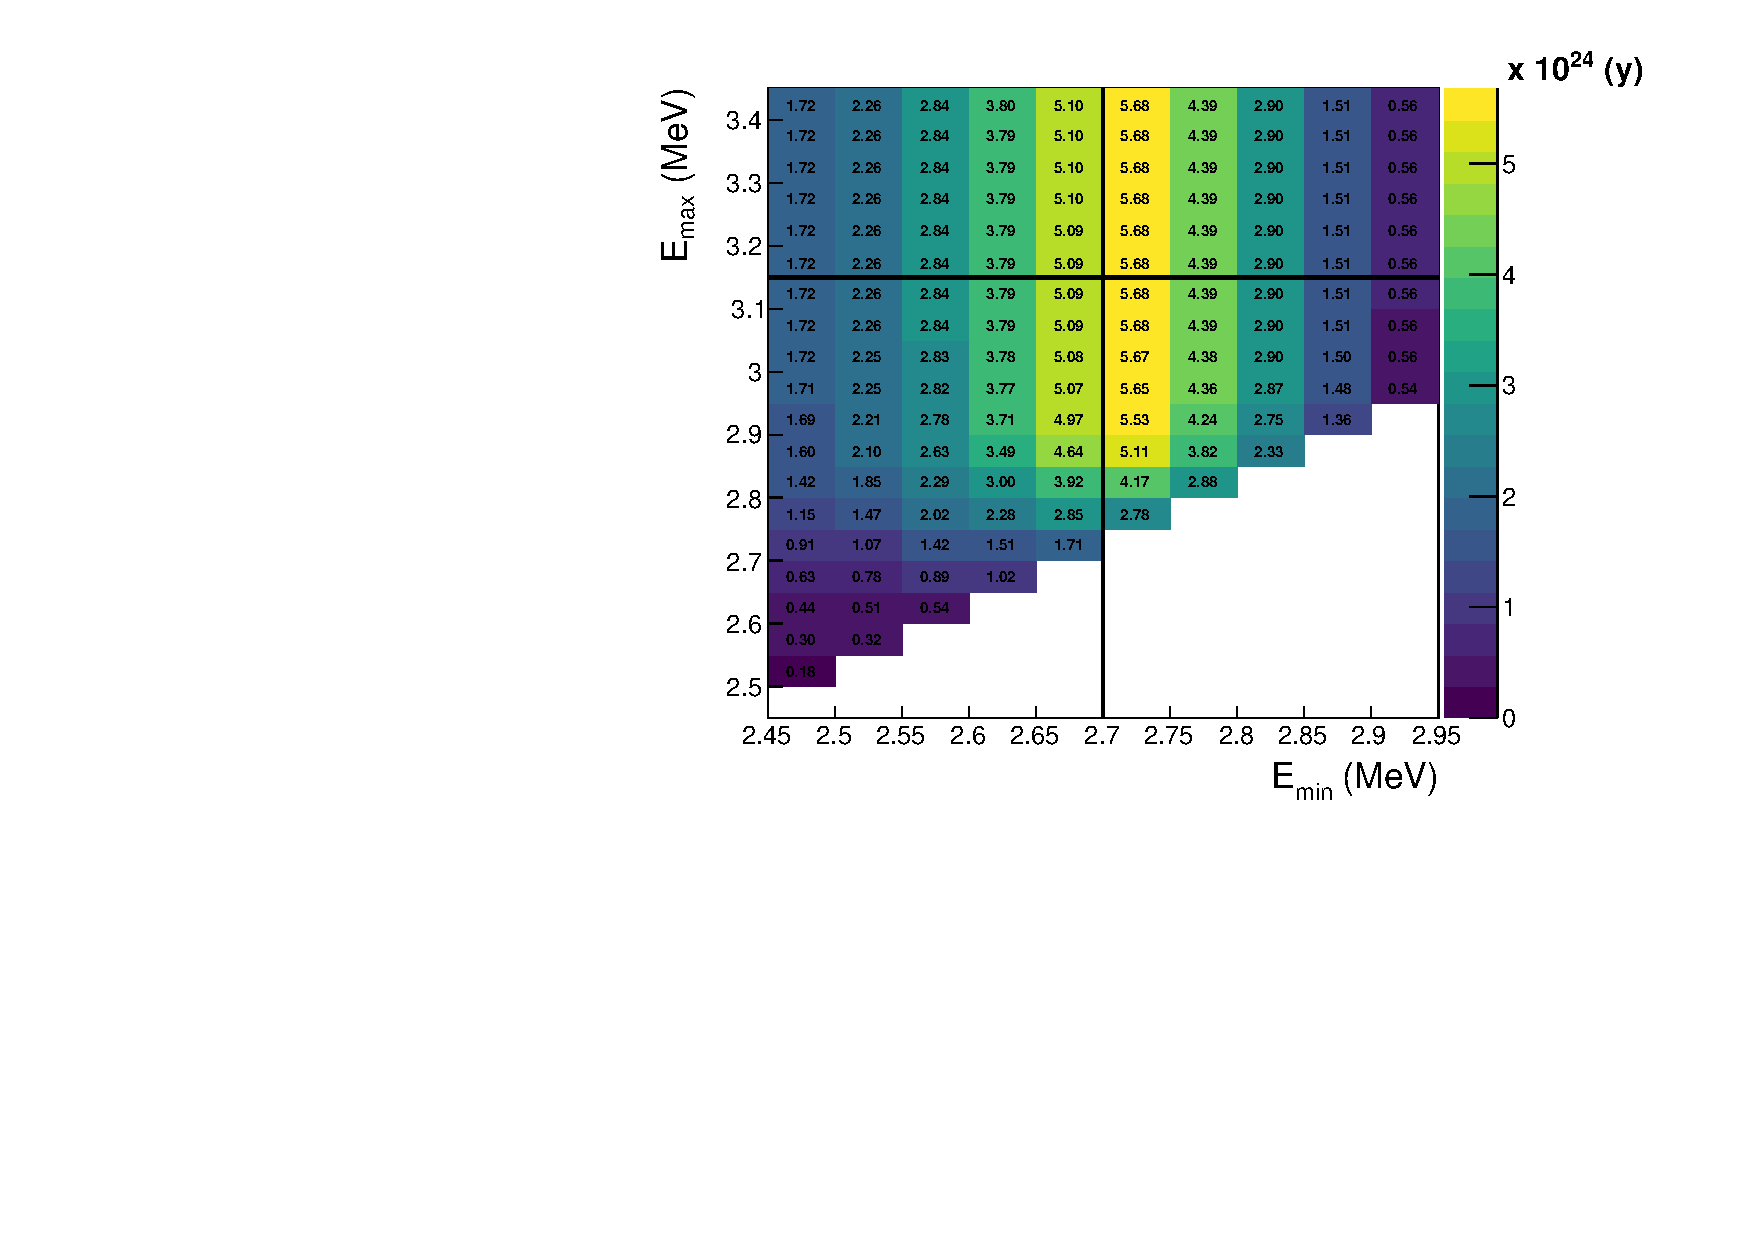
\includegraphics[width=1.1\textwidth]{Sensitivity/fig_sensitivity/sensitivity_spectrum_with_B_82Se.pdf}
  \caption{Two-dimensional histogram showing the evolution of the $\Tbeta$ value as a function of the lower and upper energy bounds.
    The maximal upper limit of $\Tbeta~>~5.7\times~10^{24}$~y (90\%~CL) is retained, in the [$2.7$;$3.15$]~MeV region of interest.
    \label{fig:sensitivity_cont}}
\end{figure}
As we said, the energy range chosen as the region of interest for the search of the $\zeronu$ decays is the one maximising the $\Tbeta$.
We found that, for the demonstrator exposure, with \Se\ sources, with a $25$ Gauss magnetic field, and for the specified background activities, the best ROI is [$2.7$;$3.15$]~MeV.
In this optimised energy range, the sensitivity expected for the SuperNEMO demonstrator stands at
\begin{equation}
\Tbeta > 5.7\times 10^{24}\,\text{y}\qquad (90\% \text{CL})\,.
\end{equation}
This result is compatible with previous SuperNEMO analysis~\cite{CalvezThesis}.

%% That work achived, we derive the expected number for each background, following Eqs.~\eqref{eq:N_2nu} to~\eqref{eq:N_Rn}, still as a function of the $\text{E}>\text{E}_{\text{min}}$ energy.
%% These are summurised in Fig.~\ref{fig:Nbackground_spectra}.
%% \begin{figure}[h]
%%   \centering
%%   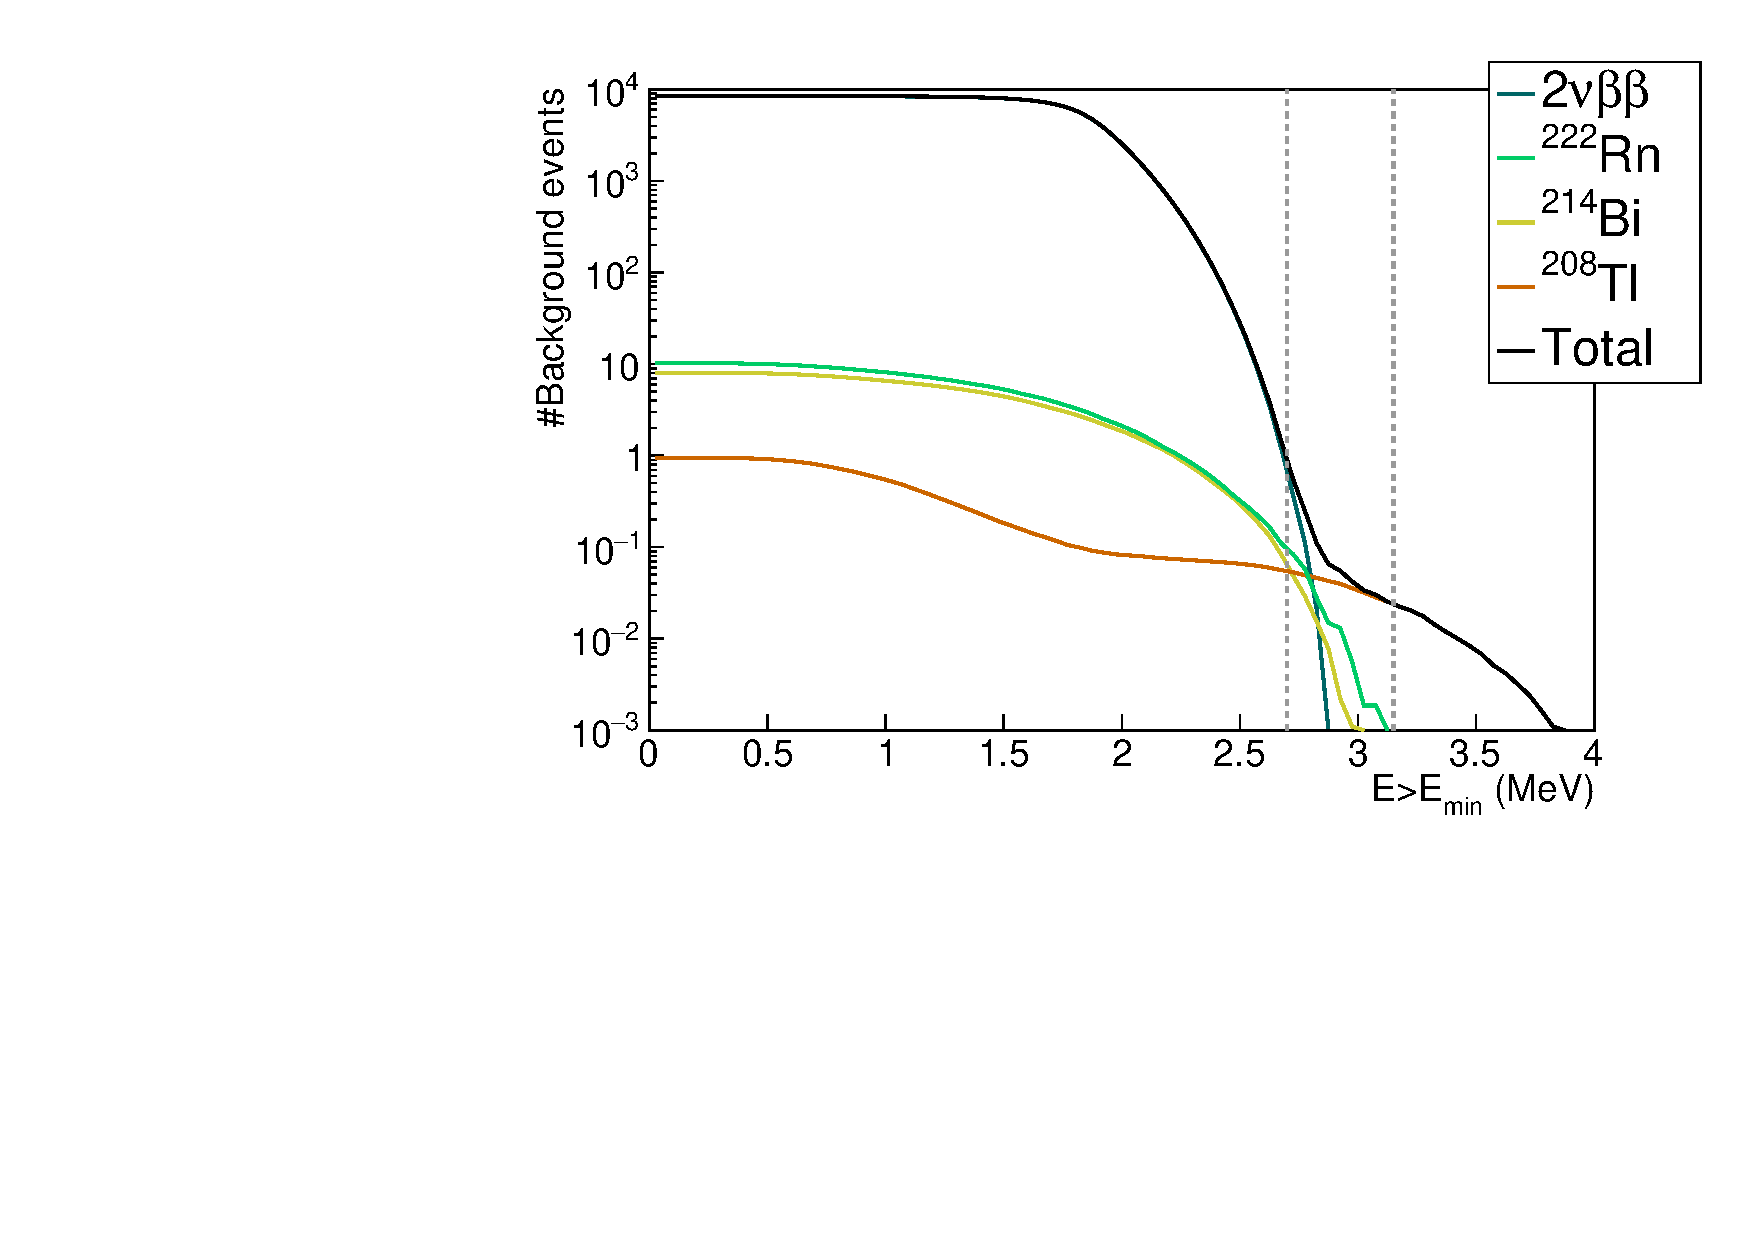
\includegraphics[width=0.8\textwidth]{Sensitivity/fig_sensitivity/Nbackground_spectrum_with_B_82Se.pdf}
%%   \caption{Expected number of background events, for $\text{E}>\text{E}_{\text{min}}$.
%%     \label{fig:Nbackground_spectra}}
%% \end{figure}

%%It depends on the exposure, on the isotope chosen for the experiment, as well as its total number of nuclei inside the source foils, all of these different conditions being detailed in the following.

\subsection{Limit on the effective neutrino mass}

The decay rate for the light Majorana exchange mechanism is given by:
\begin{equation}
  (T_{1/2}^{0\nu})^{-1} = g_{A}^{4}G^{0\nu}|M^{0\nu}|^{2}\left\lvert\dfrac{m_{\beta\beta}}{m_{e}}\right\rvert^{2}\,.
\end{equation}
where $G^{0\nu}$ is the two particles phase space factor, depending on $\Qbb$ and Z, $M^{0\nu}$ is the nuclear matrix elements for the $\zeronu$ process, and $\mbb$ is the effective Majorana neutrino mass, defined as
\begin{equation}
  \langle \mbb \rangle = \left\vert \Sigma_{i}m_{i}U^{2}_{ei} \right\vert \,,
\end{equation}
where $m_{i}$ are the neutrino masses, and $U^{2}_{ei}$ is the mixing matrix.
Therefore, the effective mass takes into account the neutrino mixing.
Consequently, observing the $\zeronu$ decay would not only prove the Majorana nature of neutrinos but, assuming the mass mechanism, could also constrain the absolute neutrino masses.
Given $g_{A}$, $G^{0\nu}$ and $M^{0\nu}$~\cite{PhysRevC.85.034316}\cite{MENENDEZ2009139}\cite{PhysRevLett.116.112502}\cite{PhysRevC.91.034304}\cite{PhysRevC.91.024613}\cite{PhysRevC.87.045501}\cite{PhysRevLett.111.142501}\cite{PhysRevC.91.024316}\cite{PhysRevC.82.064310}\cite{PhysRevC.83.034320}, we find the SuperNEMO demonstrator could reach a limit on the effective neutrino mass of
\begin{equation}
\langle\mbb\rangle = [0.24-0.47]~\text{eV}\,.
\end{equation}




\paragraph{}
In this section, we presented the general procedure leading to an optimised result on the $\Tbeta$ limit, and we gave the best limit on $\Tbeta$, driven by Eq.~\eqref{eq:tbeta_limit}, for the demonstrator case.
Thereafter, we discuss the results obtained for different detector exposures (demonstrator and final detector), and different internal background activities.
Also, and this is the main purpose of this study, we discuss the influence of the presence of the magnetic field on the final detector's sensitivity.
%%


\section{Impact of sources contamination levels on the sensitivity}
\label{sec:demonstrator_sensitivity}

We study the impact of the isotope contamination levels (inside the source foils, as well as on the tracker's wires) on the $\zeronu$ sensitivity.
We also optimise additional event selections aimed at improving the final sensitivity result.


\subsection{Influence of the contamination levels}
\label{subsec:Influence_cont}
Specified contamination levels have been established in order to achieve the $\zeronu$ half-life target of $\sim 1\times 10^{26}$~years for the final detector.
The \Se\ demonstrator source is segmented in $34$ foils, whose production was the responsibility of different laboratories (Dubna, LAPP and Tomsk).
The sources have undergone different purification treatments, in order to investigate new techniques, and to compare them with those of NEMO-$3$.
After the sources production and purification, preliminary measurements have been performed with the BiPo-$3$ detector to determine the actual \Tl\ and \Bi\ contamination levels inside the foils~\cite{internal:bipo}.
The level of radon emissions inside the tracker was also measured by the collaboration, for each of the four sections of the chamber, using a concentration line.
We summarise all these contamination levels in Tab.~\ref{tab:real_target_act}, and give a comparison with the detector initial specifications.
\begin{table}[h]
  \centering
  \begin{tabular}{|c|c|c|}
    \hline
    & Specified activities & Measured activities \\
    \hline\hline
    \Tl  & $2\,\mu$Bq.kg$^{-1}$ & $54\,\mu$Bq.kg$^{-1}$ \\
    \Bi  & $10\,\mu$Bq.kg$^{-1}$ & $<290\,\mu$Bq.kg$^{-1}$ \\
    \Rn  & $0.15$ mBq.m$^{-3}$ & $0.15\pm 0.02$ mBq.m$^{-3}$ \\
    \hline
  \end{tabular}
  \caption{Real and targeted specified activities for the SuperNEMO detector.
    The \Rn\ tracker contamination is measured with a concentration line~\cite{conf:radon2017}, extrapolated with a $2$~m$^{3}$/h flow rate.
    The limit on \Bi\ contamination is provided by BiPo measurements for a $90\%$ CL~\cite{internal:bipo}.
    \label{tab:real_target_act}}
\end{table}
The targeted \Tl\ level is not reached, being almost $27$ times higher than expected, and $3.0\times 10^{4}$ internal Thallium events are expected in $2.5$ years.
Nevertheless, on average, the activity of the sources was improved by a factor of $2$ compared to the $^{100}$Mo sources of NEMO-$3$.
In addition, valuable information has been accumulated on the different production techniques, which are of great importance for the final detector construction.
In particular, the two best \Tl\ sources activities were reached by inverse chromatography, reaching a $20\pm10~\mu$Bq/kg level, an improvement by a factor $5$ compared to NEMO-$3$.
This encourages for further investigations in this direction.
The sensitivity of BiPo detector only allowed to give an upper limit on the level of internal \Bi(an activity of $290~\mu$Bq/kg would correspond to $1.6\times~10^{5}$ internal Bismuth events in $2.5$ years).
Precise measurements are expected from the demonstrator calibration.
Radon emissions from the tracker were also measured, and extrapolated with an air flow rate of $2$~m$^{3}$/h inside the chamber, showing the targeted level of $0.15$ mBq.m$^{-3}$ was reached.
%We give in the following the influence of the contamination levels on the demonstrator's sensitivity to the $\zeronu$ decay.

In Sec.~\ref{sec:Nbkg_ROI}, we developed the general procedure allowing to set a $90\%$ confidence interval limit on $\Tbeta$.
For the demonstrator, supposing the specified activities are reached, the demonstrator would achieve a sensitivity of $5.7\times~10^{24}$~years on the searched decay, in $2.5$~years of data acquisition, with $7$~kg of \Se.
This sensitivity could be affected by the higher-than-specified level of contaminations, measured by BiPo, inside the source foils.
We expose in Fig.~\ref{fig:real_target_act} the $\Tbeta$ limit as a function of the contamination levels, as well as the corresponding chosen region of interest.
\begin{figure}[h]
  \centering
  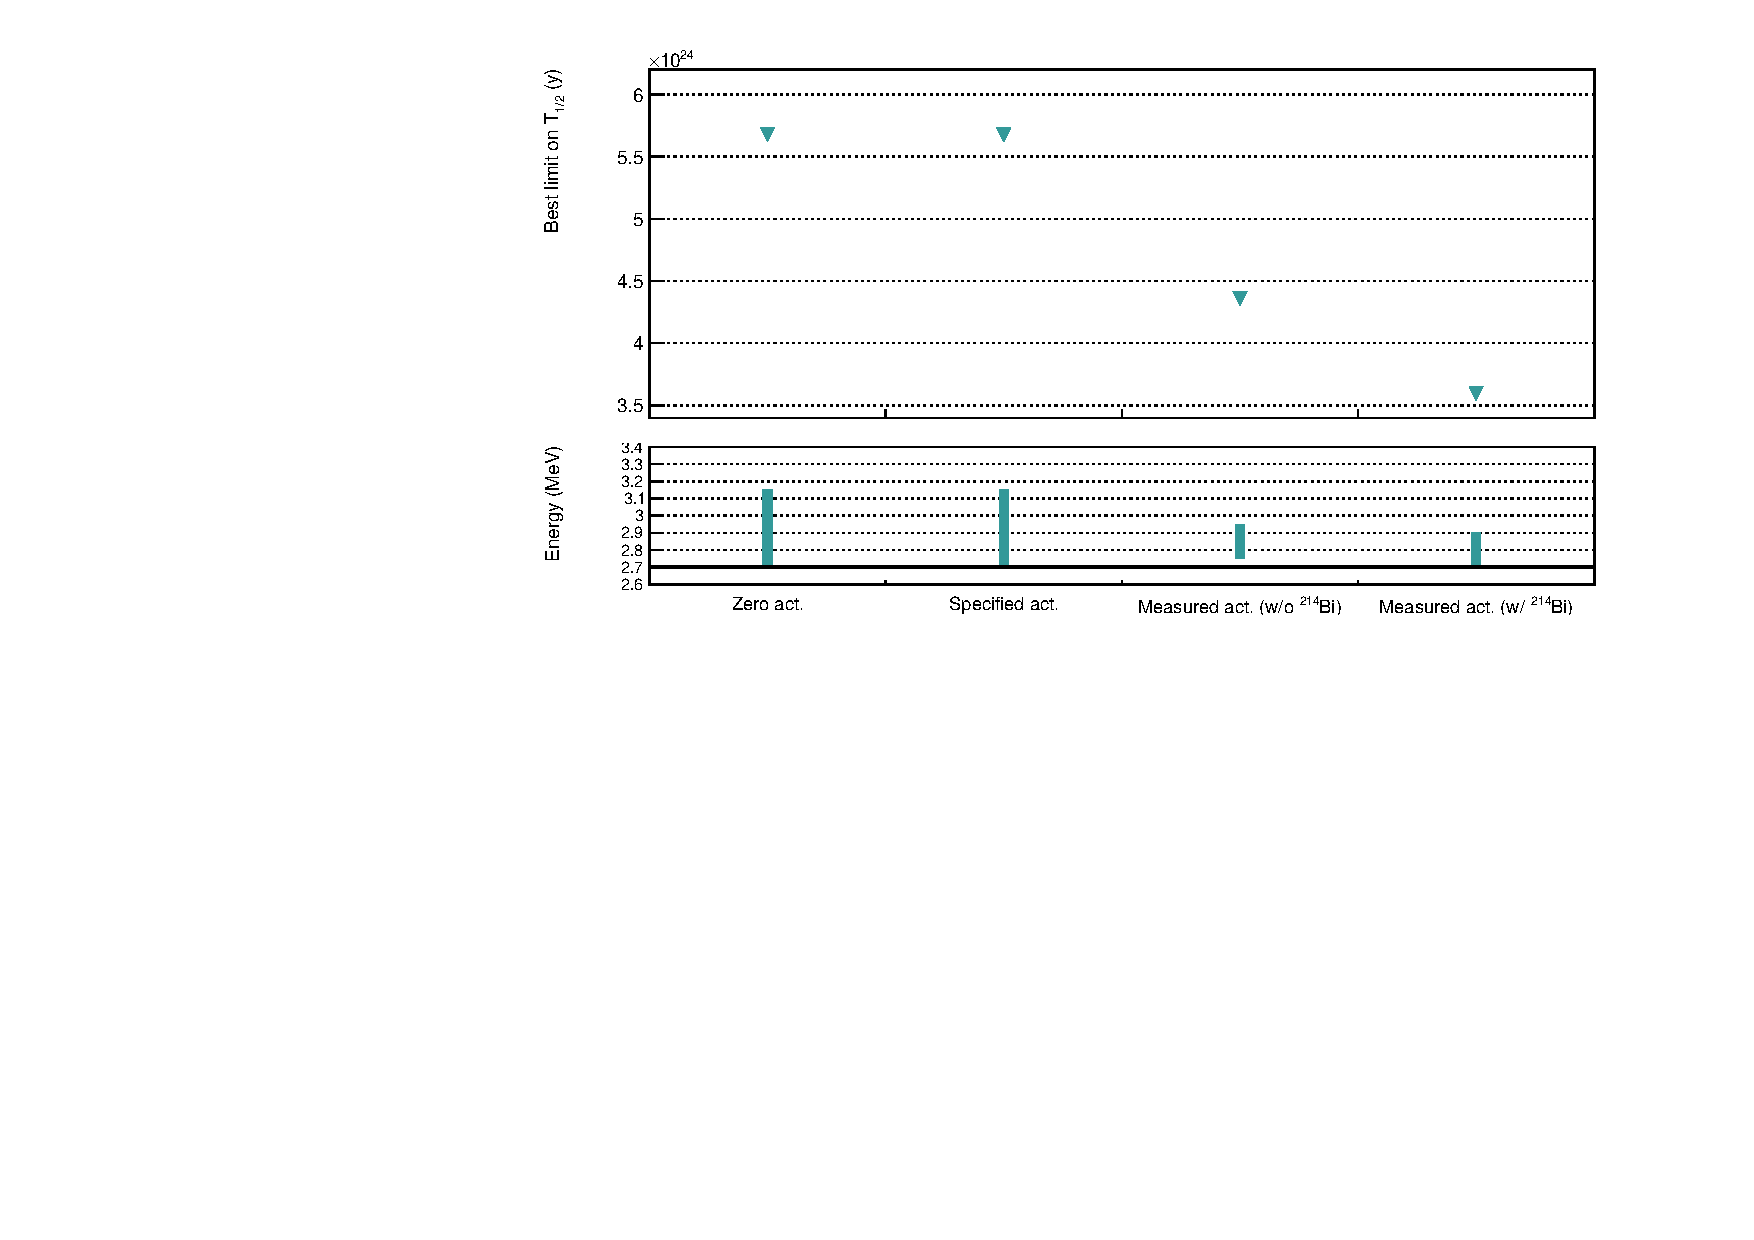
\includegraphics[width=1.1\textwidth]{Sensitivity/fig_sensitivity/contamination_level_Se_B.pdf}
  \caption{The $90\%$ CL limit on the $\zeronu$ half-life (top pad), and the corresponding ROI (bottom pad), as a function of the contamination level considered.
    For the \emph{zero activities} case, we consider hypothetical contamination levels where $\mathcal{A}^{\text{Bi}}~=~\mathcal{A}^{\text{Tl}}~=~0~$Bq/kg.
    The \emph{specified activities} are presented in Tab.~\ref{tab:real_target_act}.
    The \emph{measured activities}, provided by the BiPo detector~\cite{internal:bipo}, are presented in the same table.
    We consider successively a null \Bi\ contamination (\emph{measured act. w/o \Bi}), or equals to the $290\mu\,$Bq/kg upper limit (\emph{measured act. w/ \Bi}).
    \label{fig:real_target_act}}
\end{figure}
%% For each level, we oppose two distinct magnetic field cases: a $25$~G magnetic field, or no field.
%% In the current sub-section, we focus on the comparison between different contamination levels.
%% The conclusions about the presence of the magnetic field we will be discussed in the next sub-section.
Four distinct levels of internal contaminations are considered:
\begin{itemize}
\item the \emph{zero activities} case, a hypothetical case where the source foils and the tracker are non contaminated at all,
\item the \emph{specified activities} case, were the targeted level of contaminations would have been reached,
\item and two \emph{measured} cases, that take into account the measured levels of contaminations at $90\%$ CL.
  As the \Bi\ activity is provided by BiPo measurements as an upper limit, it is possible for this level to be lower than $290\,\mu$Bq/kg.
  We therefore present the results, either for sources that would not be contaminated by this isotope (the \emph{without \Bi} case), or considering that the activity reached is $290\,\mu$Bq/kg (\emph{with \Bi}).
\end{itemize}
The fact that we are showing results for a hypothetical zero isotope contamination is to illustrate an important statistical phenomenon.
Indeed, we notice that there is no difference in sensitivity, or ROI, between the first two cases of contamination, which may seem surprising at first glance. %%$1.6e5$
This is explained by the Feldman-Cousins statistics employed to determine the number of excluded signal events, $N_{0\nu}^{\text{excl.}}$, given the number of observed background events (defined from Eq.~\eqref{eq:N_2nu} to Eq.~\eqref{eq:N_Rn}).

\paragraph{Clarifications on Feldman-Cousins statistics}
When the expected number of background events is negligible (which is the case for the two first levels presented), the probability $p$ to observe $n_{s}$ signal events, expecting $s$ events, is given by the Poisson distribution
\begin{equation}
p = \frac{e^{-s}s^{n_{s}}}{n_{s}!}\,.
\end{equation}
Let's now put ourselves in the situation where no signal event is observed - that is what we assume to put an upper limit on the $\zeronu$ half-life.
Then $n_{s}\rightarrow~0$, and $p\rightarrow~e^{-s}$.
If zero signal event is \emph{observed}, it is uncorrect to assume that zero signal events were \emph{produced} during the experiment.
We only can say that no signal event has been observed \emph{a priori}.
To account for this particular case, the quantity $s$ should no longer be viewed as the number of expected signal events, but as the number of excluded signal events, $N_{0\nu}^{\text{excl.}}$.
In the end, for a negligible expected number of background events, and no signal event observed, we can set an upper limit on the number of excluded signal events, excluding values for which $p < \alpha$.
Taking a $90\%$ confidence interval, that is to say $\alpha~=~10\%$, we obtain $s \leq 2.303$.
A direct consequence of this statement is, considering that the background levels for the two first cases are negligible (or null) in the region of interest, they both reach this limit of $2.303$ on the excluded number of signal events.
Therefore, due to the Feldman-Cousins statistics, no difference is observed in terms of half-life limits between these two contamination cases.
%% To help visualise the situation, we show in Fig.~\ref{} the distribution of $N_{0\nu}^{\text{excl.}}$, for the demonstrator case, for the two first contamination cases.
%% \begin{figure}[h]
%%   \centering
%%   \includegraphics[width=1.1\textwidth]{Sensitivity/fig_sensitivity/}
%%   \caption{
%%     \label{fig:}}
%% \end{figure}

\paragraph{}
When considering the measured internal activities, a decrease in sensitivity is observed, compared with the specified activities case.
Indeed, the number of background events in the ROI is no more negligible, and influence significantly the value of $\Tbeta$, decreasing the experiment's sensitivity by $23\%$ (without \Bi) and $37\%$ (with \Bi).
Both region of interests are also highly reduced, especially for the third contamination case, where the lower bound is greater than $2.7$~MeV, an energy region populated with a non-negligible number of background events.
This impacts significantly the signal-to-background ratio, as addressed in the next sub-section~\ref{subsec:opti_ev_selection}.

The degradation of the limit with the level of contamination remains acceptable.
However, we can try to improve the situation by exploring new event selection techniques, with the aim of maximising the limit on $\zeronu$ half-life.

\begin{itemize}
\item préciser que si ça se trouves les niveaux de cont. sont plus élevés que ça, car pas toutes les sources ont été mesurées, et que certaines valeurs sont des limites sup.
\end{itemize}

\subsection{Optimisation of the event selection}
\label{subsec:opti_ev_selection}

The measured level of \Tl\ isotope inside the source foils is greater than the specifications.
Moreover, an upper limit, higher than the specified level for SuperNEMO, has been set by the BiPo detector, regarding the internal \Bi\ level.
Consequently, we can imagine implementing stricter cut-offs, to reject a background level higher than the specifications.
Most of the double beta experiments are only sensitive to the total electron energy sum.
The unique SuperNEMO tracko-calo technology confers the experiment the ability to characterise single particles (individual energies, emission angles...).
Based on previous studies~\cite{CalvezThesis}~\cite{ChaponThesis}, \emph{topological cuts}, relying on these additional observables, have been set up.
They are especially designed to reject events where the two electrons are not emitted simultaneously, or from the same location on the source foils.

\paragraph{The internal probability}
Based on time-of-flight (TOF) computation, the internal probability (\Pint) is derived from the internal $\chi^{2}$ (see details in Sec.~\ref{subsec:internal_prob}).
In Fig.~\ref{fig:Pint} are presented the internal probability spectra for the $\zeronu$ signal and all background processes, after the first-order selections.
\begin{figure}[h]
  \centering
  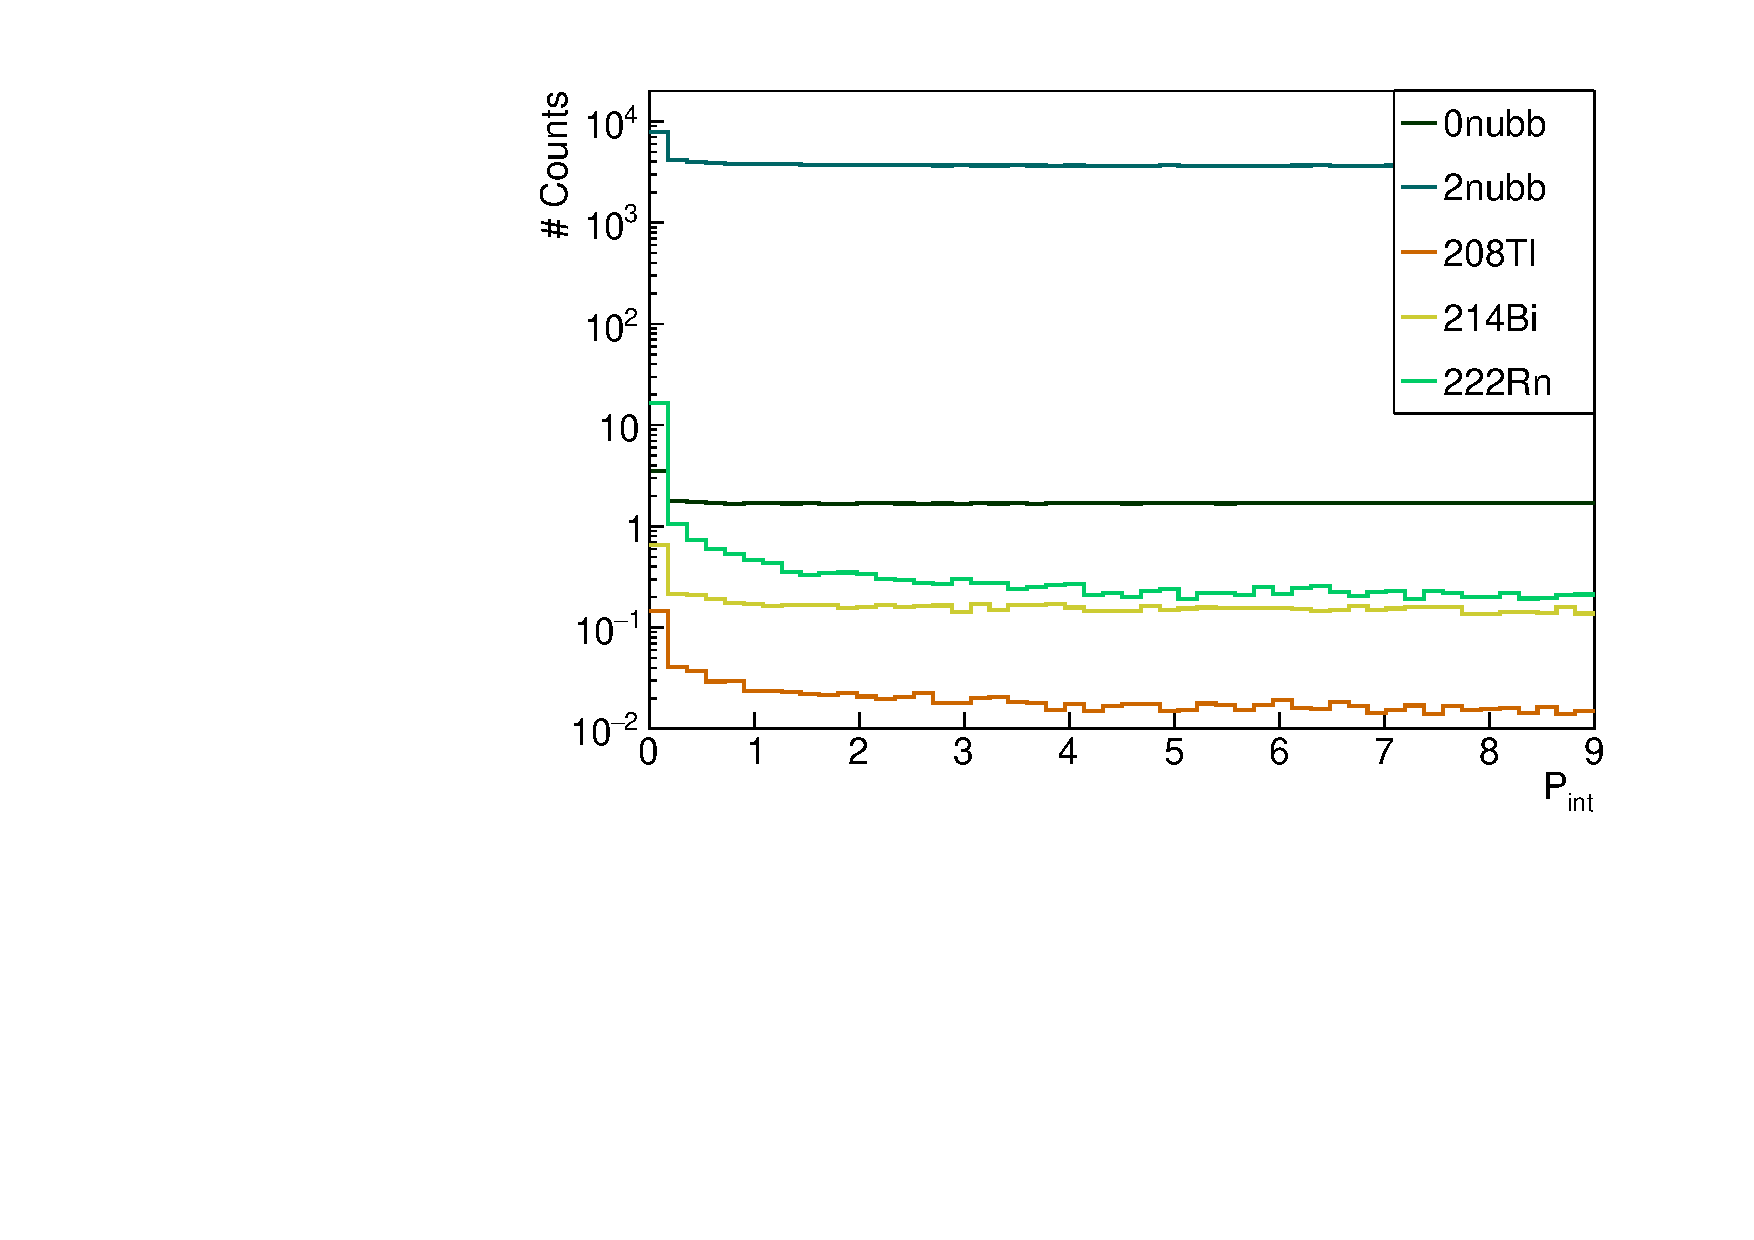
\includegraphics[width=0.8\textwidth]{Sensitivity/fig_sensitivity/InternalProbability.pdf}
  \caption{Internal probabilities for all processes.
    First-order cuts have been applied.
    $\beta\beta$ distributions are normalised to the half-lives, and background processes are normalised to the specified activities.
    \label{fig:Pint}}
\end{figure}
These distributions are normalised to the double beta half-lives, and the nominal activities.
Equivalent distributions, but with different \Bi\ and \Tl\ contamination levels, can be derived for the case of measured activities.
The internal probability distributions for the $\zeronu$ and $\twonu$ processes follow the expected flat distribution for electrons emitted simultaneously from the source.
As the disintegration of Bismuth actually takes place from the sources, the \Bi\ distribution is also flat.
The same could have been assumed for Thallium, however, the distribution is distorted at low internal probabilities.
This might be explained by the existence of a metastable excited state ($\tau_{1/2} = 294 ps$) of the daughter nuclei, which would slightly delay the second electron emitted via internal conversion.
This feature is addressed in detail in Chap.~\ref{ch:timediff}.
The Radon, being a non-internal background, presents a peak at low internal probabilities.

We want to evaluate the influence of a cut-off on the simulations using internal probability as a rejection criterion: simulated events are selected for \Pint\ values upper than a given limit.
The standard value applied in NEMO-$3$ analyses was \Pint~$>~4~\%$.
We wish to establish the most adequate \Pint\ selection level for the SuperNEMO demonstrator.
%The signal and background selection efficiencies then depend on the contamination activities considered.
For each internal probability cut-off applied to the simulations, we evaluate the $\Tbeta$ at a $90$~\% confidence interval, as well as the best ROI.
The internal probability value that will be chosen will be the one that maximises the sensitivity, and depends on the internal level of contamination.
To better understand this optimisation, let us present the $\epsilon_{0\nu}$ values for each \Pint\ selection case, in Fig.~\ref{subfig:cont_Pint_eff}, both for the specified and measured contamination levels.
\begin{figure}[!h]
\centering
\begin{subfigure}[t]{0.49\textwidth}
  \centering
  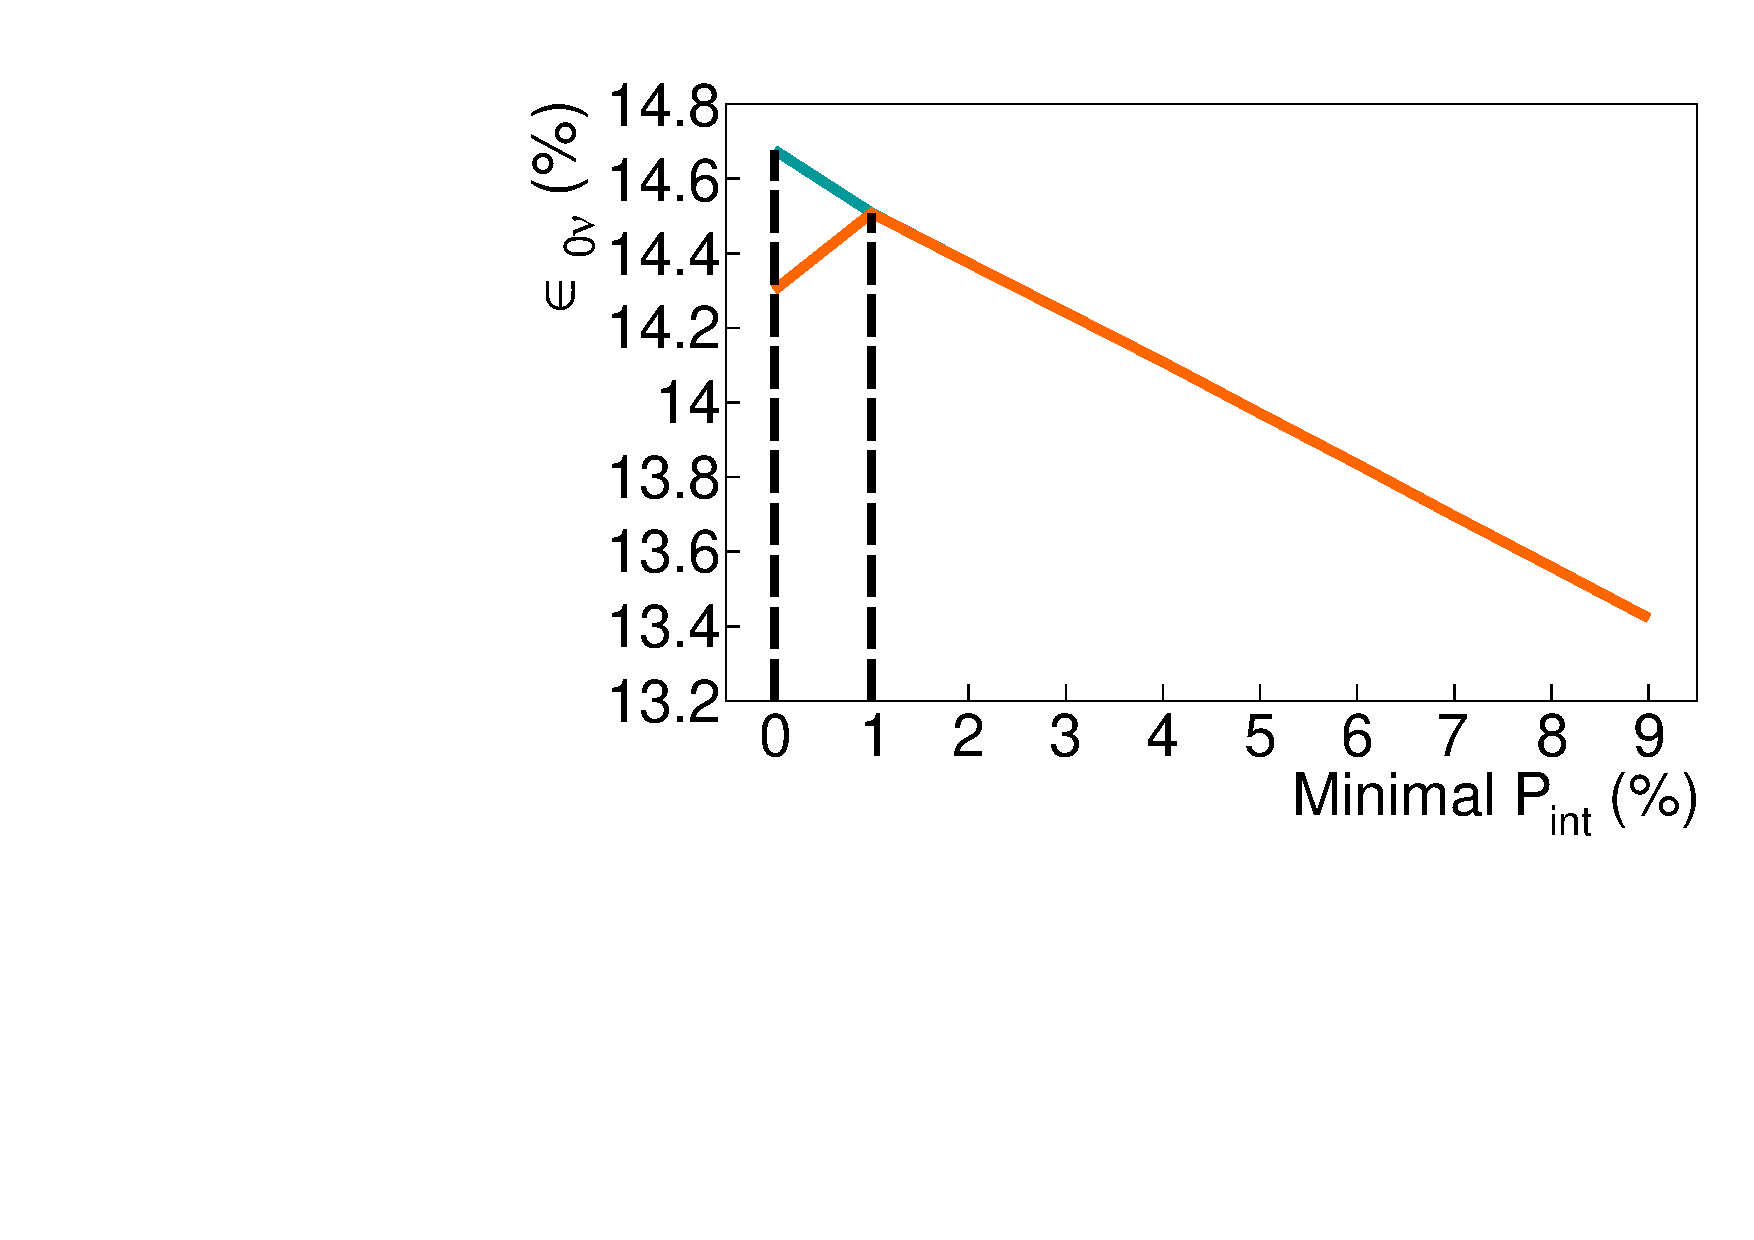
\includegraphics[width=0.82\textwidth]{Sensitivity/fig_sensitivity/cont_cut_eff_B.pdf}
  \captionsetup{justification=justified}
  \caption{
    \label{subfig:cont_Pint_eff}}
\end{subfigure}
\hfill
\begin{subfigure}[t]{0.49\textwidth}
  \centering
  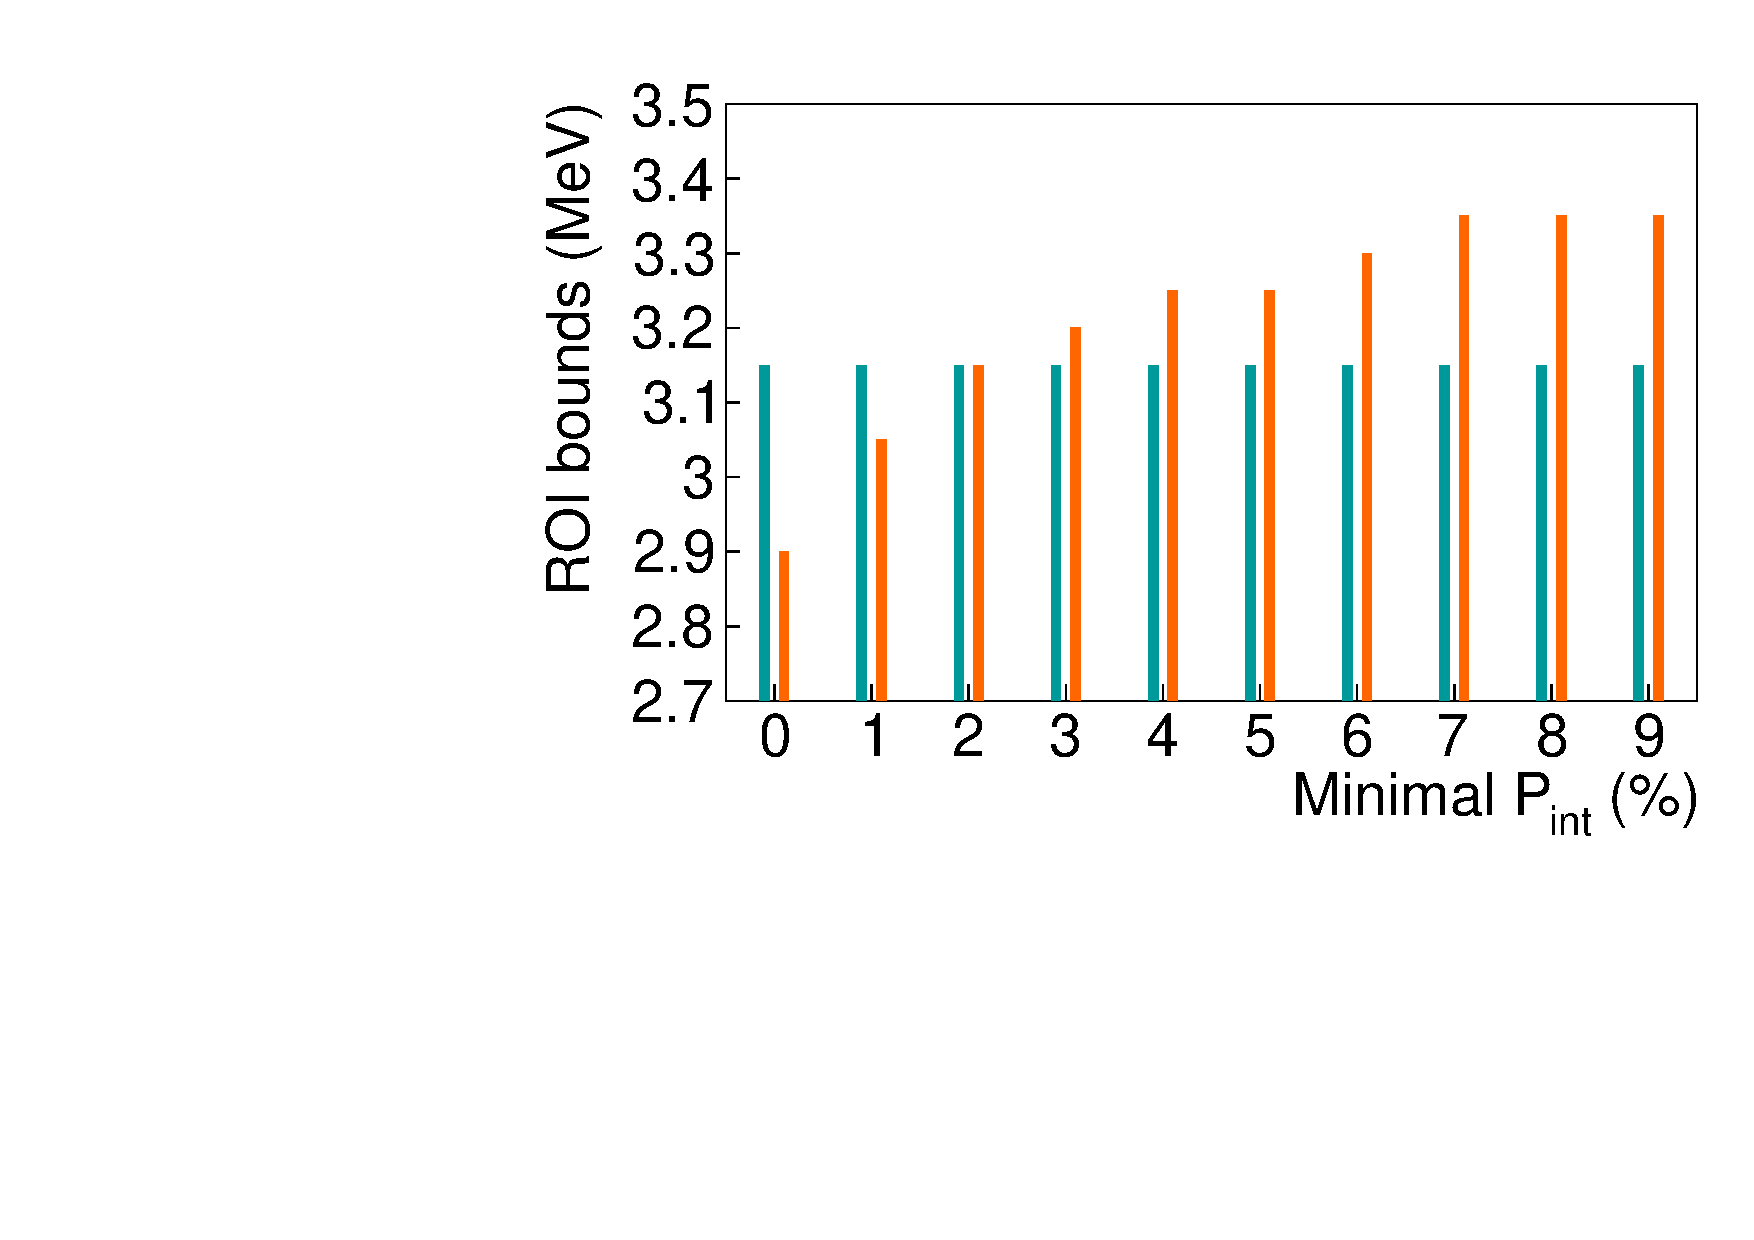
\includegraphics[width=0.82\textwidth]{Sensitivity/fig_sensitivity/ROI_cut_Pint_B.pdf}
  \captionsetup{justification=justified}
  \caption{
    \label{subfig:cont_Pint_ROI}}
\end{subfigure}
\vskip\baselineskip
\begin{subfigure}[t]{0.49\textwidth}
  \centering
  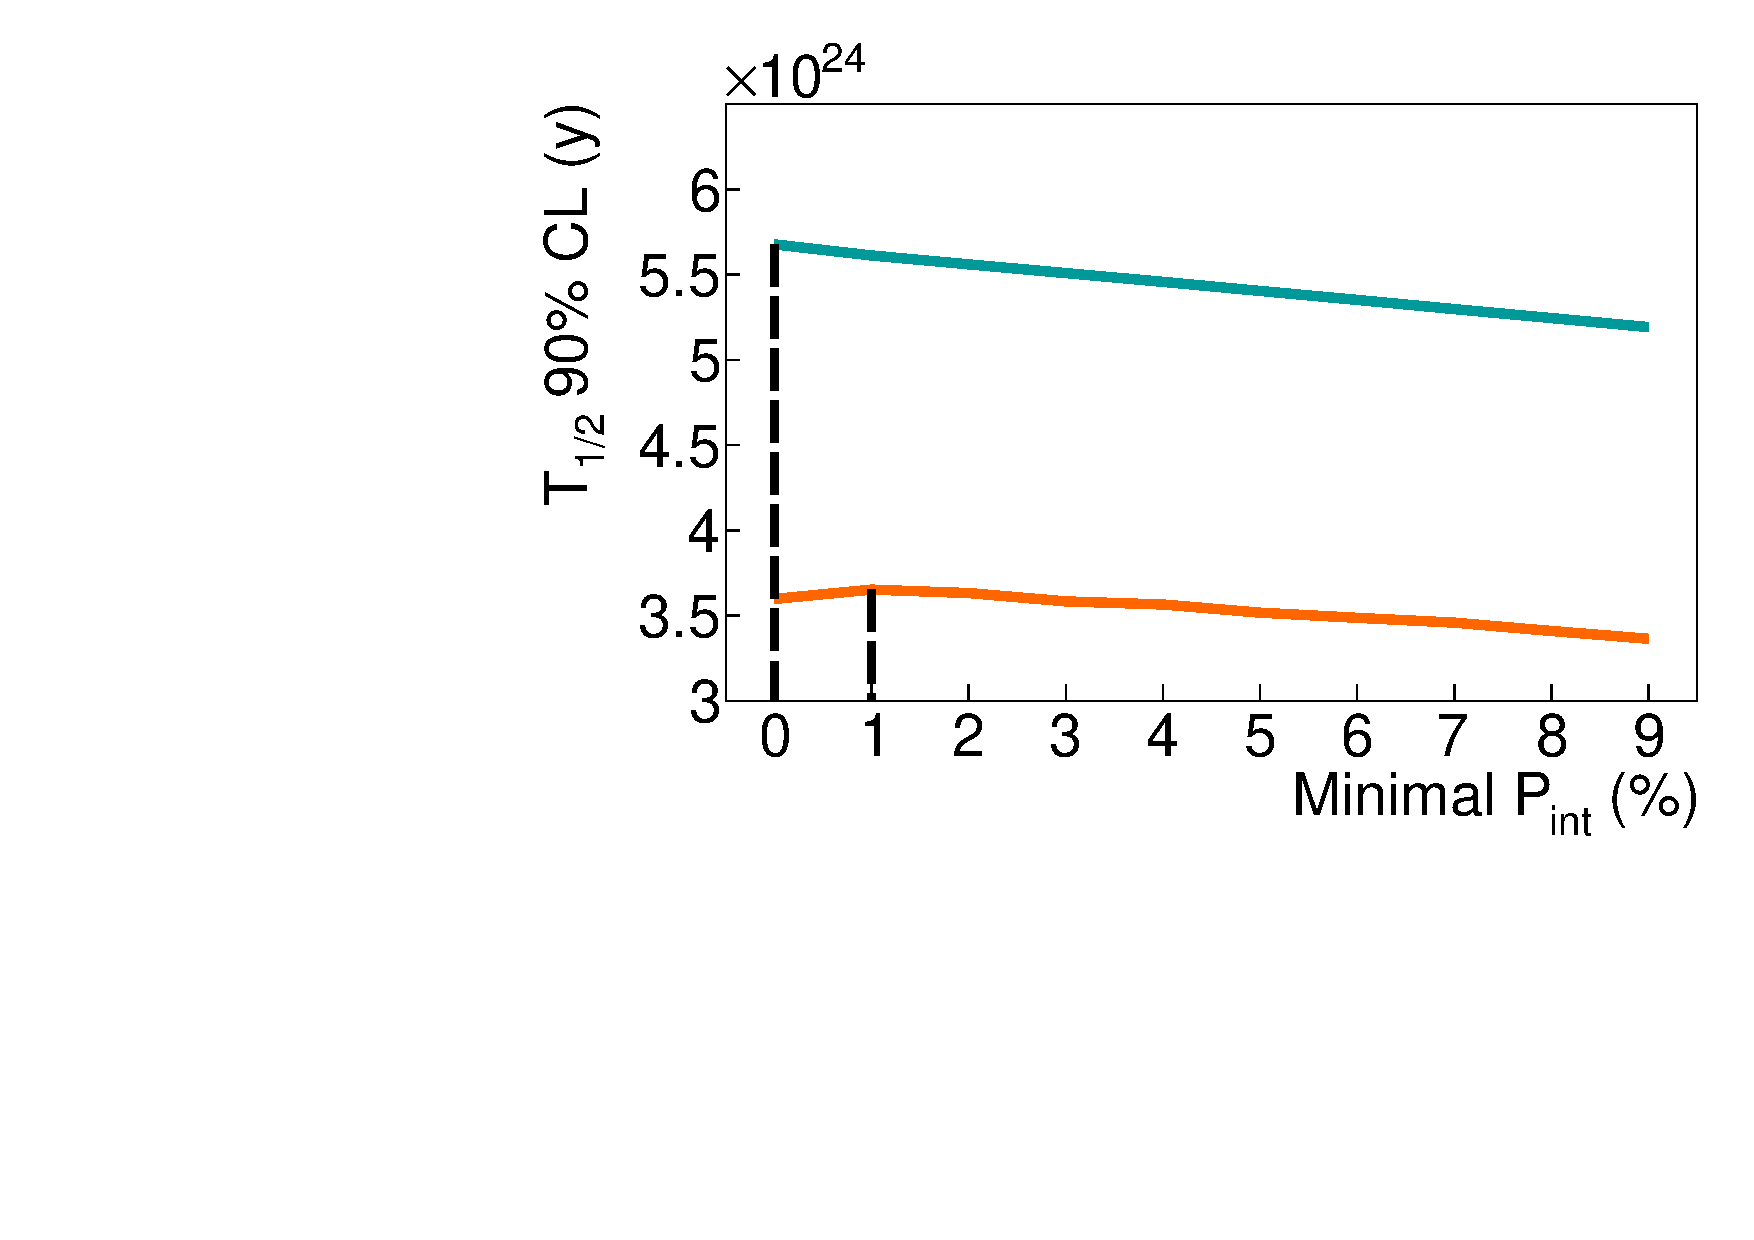
\includegraphics[width=0.82\textwidth]{Sensitivity/fig_sensitivity/cont_cut_T12_B.pdf}
  \captionsetup{justification=justified}
  \caption{
    \label{subfig:cont_Pint_T12}}
\end{subfigure}
\hfill
\begin{subfigure}[t]{0.49\textwidth}
  \centering
  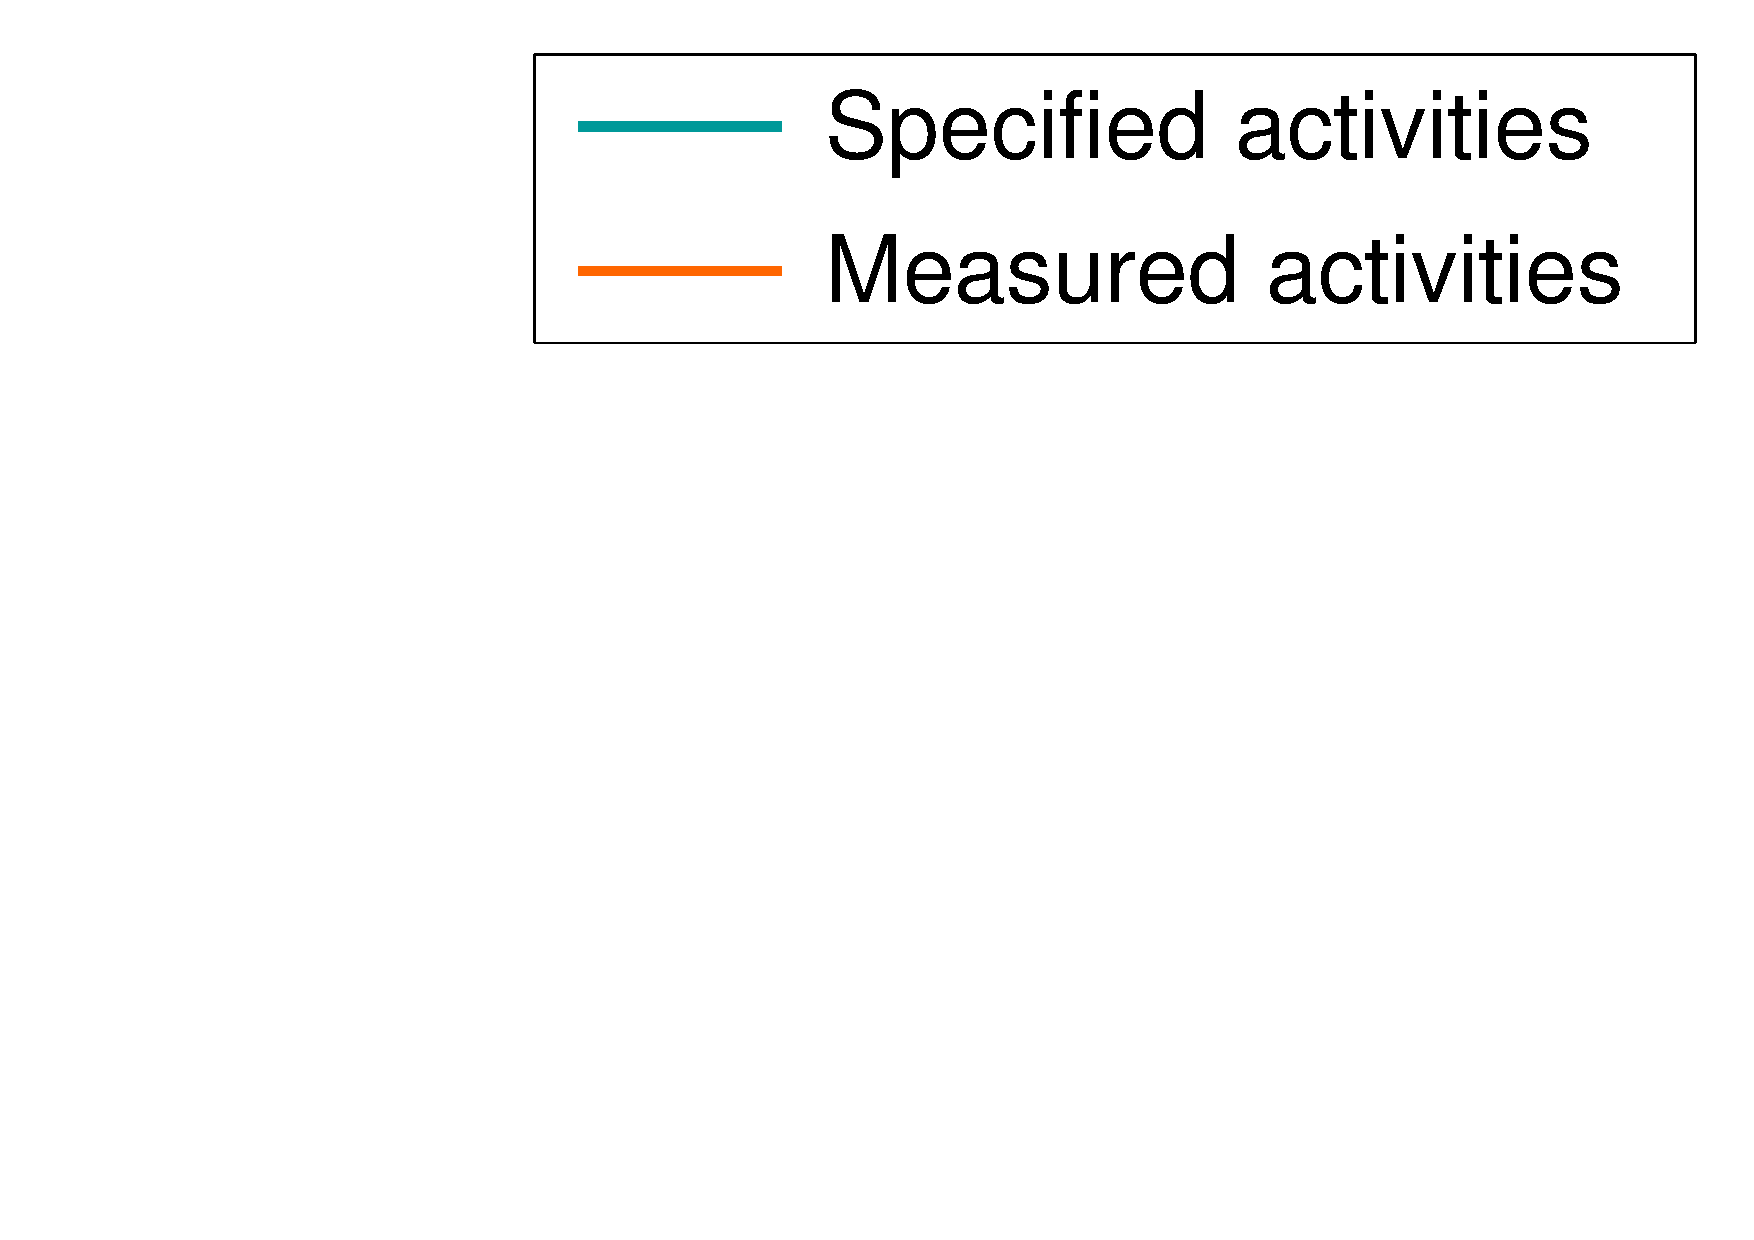
\includegraphics[width=0.82\textwidth]{Sensitivity/fig_sensitivity/legend_cut_Pint.pdf}
  \end{subfigure}
\caption{The $\zeronu$ selection efficiency, $\epsilon_{0\nu}$ (a),
  evolution of the region of interests (b),
  and best limits set on $\Tbeta$ at $90\%$ CL, as a function of the cut-off applied on internal probability, \Pint.
  Results are displayed for two contamination levels: the specified (blue) and the measured (orange) activities.
  An exposure of $17.5$~kg.y is considered.
  Two vertical dashed lines in (a) and (c) display the best \Pint\ selections to be applied in order to improve the $\Tbeta$ sensitivity of the experiment.
  \label{fig:cont_Pint}}
\end{figure}
For the latter, we assume the Bismuth upper limit of $290~\mu$Bq/kg activity is reached.
As expected, in both cases, the $\epsilon_{0\nu}$ selection efficiency globally decreases with the \Pint\ cut-off applied.
However, for the measured contamination case, we observe a slight increase of the $\zeronu$ selection efficiency, for \Pint\ $>~1~\%$.
Fig.~\ref{subfig:cont_Pint_ROI}, showing the variations of the regions of interest as a function of the \Pint\ rejection criterion, allow to understand this observation.
For the measured activities case, from the level \Pint~$>~0~\%$ to \Pint~$>~1~\%$, the ROI upper bound increases from $2.9$ to $3.05$~MeV.
Usually, the variation of this bound does not have such a great impact on the event selection.
%, as very low number of background and signal events are expected at high energies (see Fig.~\ref{fig:energy_spectra}).
Nevertheless, in the measured activities case, for a \Pint~$>~0~\%$ level, the ROI is optimised at the narrow [$2.7$;$2.9$]~MeV interval, where the upper bound is located in an energy region still populated by signal and bakground (see Fig.~\ref{fig:real_target_act}).
Therefore, even small variations in this ROI has a great impact on the results, explaining the local increase in efficiency.
For \Pint\ selections greater than $1~\%$, we come back in cases where the upper limit of the ROI no longer has an impact on $\epsilon_{0\nu}$.
For the specified ativities case, the ROI bounds are stable, not impacting the selection efficiency.

%% Indeed, the amount of background event selected varies with the \Pint\ cut-off value.
%% This number has a strong influence on the chosen region of interest, as explained in Sec.~\ref{sec:Nbkg_ROI}.
As the limit set on $\Tbeta$ depends directly on $\epsilon_{0\nu}$, the variations presented in Fig.~\ref{subfig:cont_Pint_eff} fully explain the results displayed in Fig.~\ref{subfig:cont_Pint_T12}, presenting the evolution of $\Tbeta$ with the internal probability selection level.
The sensitivities displayed for a $0\%$ cut-off on P$_{\text{int}}$ of course correspond to the results given in Fig.~\ref{fig:real_target_act}.
%We conclude that with low background constraints, the internal probability cut-off only decreases the sensitivity to the $\zeronu$ decay.
The main conclusion is that this rejection criterion has only a limited impact on the improvement of $\Tbeta$ sensitivity, because of the very low contamination levels considered.
Indeed, paradoxically, the selection on internal probability worth it only if there is enough background events to be rejected.
The former $4~\%$ value recommended by the NEMO-$3$ analysis is then too high for the SuperNEMO source contamination.

%%, and we start to see the usefulness of this cut-off when we take into account the measured activities.
%% Tab.~\ref{tab:cut_Pint} summarises the best internal probability cut-off to be applied in each contamination case, as well as the corresponding sensitivity achieved.
%% \begin{table}[h]
%%   \centering
%%   \begin{tabular}{|c|c|cc|}
%%     \hline
%%     Activity & Optimised P$_{\text{int}}$ cut-off &\multicolumn{2}{c|}{$\Tbeta$ (y)}  \\
%%     &&Before cut-off&After cut-off\\
%%     \hline\hline
%%     Specified & $0\%$  & $5.7\times 10^{24}$ & $5.7\times 10^{24} (\nearrow 0\%)$  \\
%%     Measured w/o \Bi & $3\%$ & $4.4\times 10^{24}$ & $5.4\times 10^{24} (\nearrow 23\%)$ \\
%%     Measured w/ \Bi & $1\%$ & $3.6\times 10^{24}$ & $3.6\times 10^{24} (\nearrow 0\%)$ \\
%%     \hline
%%   \end{tabular}
%%   \caption{The optimisation of internal probability selection is presented for each background case.
%%     The corresponding limit on $\Tbeta$ at $90\%$ level, before and after the P$_{int}$ cut-off, is given.
%%   \label{tab:cut_Pint}}
%% \end{table}

NEMO-$3$ analyses also used the distance between the reconstructed vertices on the source foils as a background rejection criterion.
As we shown that the additional \Pint\ cut-off is poorly adapted for the low activities of SuperNEMO sources, it is interesting to know if we can improve the results by using this second selection.

\paragraph{Vertices distance}
As discussed in Sec.~\ref{sec:sensitivity_ev_selection}, an electron is defined as a reconstructed track inside the wire chamber, with one extremity on a calorimeter block, and another on a source foil.
Therefore, the $2e$ topology involves two distinct calorimeter hits, two reconstructed tracks, and two foil vertices.
Thanks to the trajectory fitting algorithm, we have access to the ($Y,Z$) coordinates of the latter, and by extension, to the distance between them.
In the previous studies, the choice was made to look at the effect of this selection, separately on the $Y$ (perpendicular to the wires) and $Z$ (paralel to the wires) directions.
We choose to follow the same approach, and we give the results for a cut along the $Z$ axis, but the conclusions remain valid for the $Y$ direction.
Fig.~\ref{fig:vertex_dist} shows the distributions of the absolute value of the distance between foil vertices for each process studied.
\begin{figure}[h]
  \centering
  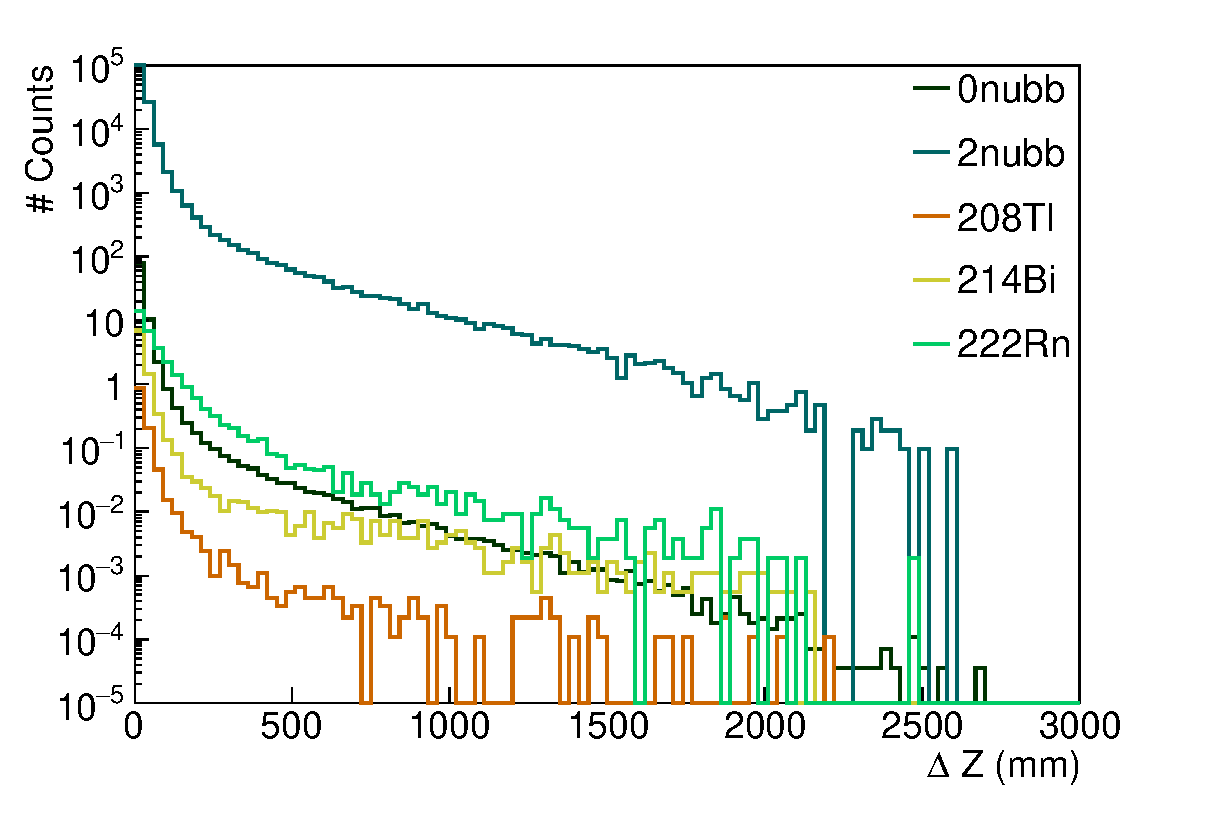
\includegraphics[width=0.8\textwidth]{Sensitivity/fig_sensitivity/Vertex_distance.eps}
  \caption{Distance between vertices along the $Z$ direction, $|\Delta Z|$, for each process considered.
    \label{fig:vertex_dist}}
\end{figure}
%% The two electrons of $\zeronu$ and $\twonu$ decays are actually emitted from the same vertex, unlike natural isotope disintegrations.
%% * a finir*
We would use this information in order to maximise the double $\beta$ decays to be selected, while rejecting natural isotope disintegrations.
%% The two reconstructed vertices on source foils should not be separated by more than $60$ mm horizontally ($|\Delta y| < 60$ mm), and by more than $70$ mm vertically ($|\Delta z| < 70$ mm), to maximise the selection of two electrons emitted at the same spot.
%% These topological cuts have to be adjusted to match the contamination levels presented in Tab.~\ref{tab:real_target_act}.

Fig.~\ref{fig:cont_vertex} displays the limit set on $\Tbeta$ as a function of this event selection, allowing to study the impact of the vertices distance cut-off on the final sensitivity.
\begin{figure}[h]
  \centering
  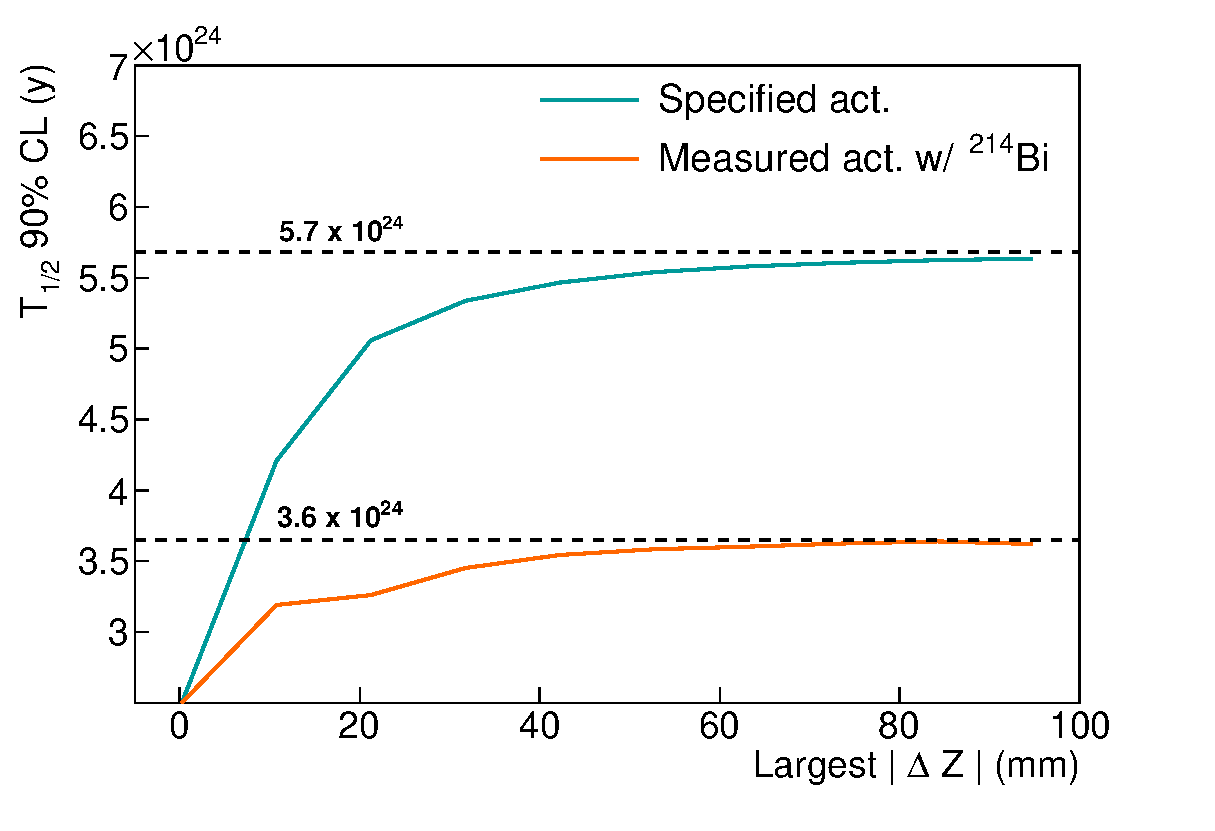
\includegraphics[width=0.8\textwidth]{Sensitivity/fig_sensitivity/contamination_vertex.eps}
  \caption{Best reached limit on $\Tbeta$, as a function of the cut-off applied on the $Z$ distance between vertices, $|\Delta Z|$.
    Results are displayed for specified (blue), and measured contaminations (with the \Bi\ contamination (orange) or without it (green)).
    No improvement in sensitivity is obtained with this event selection.
    \label{fig:cont_vertex}}
\end{figure}
In the same way as previous paragraph, we study the influence of the level of contaminations by showing results for the two specified and measured activities.
The two distributions reach a plateau, corresponding to the sensitivities achieved with the first-order cuts (Fig.~\ref{fig:real_target_act}).
Regardless of the level of contamination, the number of background events is too low in the ROI for the $| \Delta Z|$ cut-off to be worthwhile.
Therefore, the cut-off only degrades the sensitivity, as does the selection on internal probability.
The same conclusions apply to the $| \Delta Y |$ cut-off.

However, such a cut-off could be useful for rejecting unexpected background (where two electrons are emitted from two independent sources, for instance).
For example, we note that a cut-off at $|~\Delta Z~|~<~80$~mm does not significantly degrade sensitivity.
In practice, a selection on vertex distance will always be applied, even if it is very loose.

\paragraph{}The idea of having implemented these two selections (on the internal probability and on the distance between vertices) comes from a previous NEMO-$3$ analysis on the background rejection.
However, the levels of contaminations we are dealing with, is remarkably low for most of the the topological cut-offs to be worth applying.
Finally, the best \Pint\ level to be applied depends on the source activities.
Moreover, the cut-off on vertex distance is kept for $|~\Delta~Z~|~<~80$~mm (samely for $|~\Delta~Y~|$).
For future studies, it is useful to know the efficiencies of selection of these cut-off, for the signal and for each background considered.
Those are given in Tab.~\ref{tab:Pint_eff}, for the first-order cuts, a $>~1\%$ internal probability level, and a loose cut on vertices distance.
\begin{table}[h]
  \centering
  \begin{tabular}{|c|c|c|c|}
    \hline
    Process & First-order cuts (\%) & Internal probability (\%) & Vertex distance (\%) \\
    \hline\hline
    $\zeronu$  & $26.9$ & $26.2$ & $25.4$ \\
    $\twonu$  & $9.15$ & $8.90$ & $8.51$ \\
    \Tl  & $0.106$ & $0.0955$ & $0.0905$ \\
    \Bi  & $0.168$ & $0.158$ & $0.149$ \\
    \Rn  & $0.0177$ & $8.99\times~10^{-3}$ & $5.94\times~10^{-3}$ \\
    \hline
  \end{tabular}
  \caption{Selection efficiencies (number of selected $2e$ topologies compared with the total number of simulated decays), for the three levels of selection (first-order, \Pint\ and vertex distance), in the full energy range.
  \label{tab:Pint_eff}}
\end{table}
The topological cuts have a huge impact on Radon selection, as they are especially designed to reject non-internal events.
They are also efficient in rejecting Thallium internal events, because of the existence of a metastable exited state, described earlier.

After the topological cut-off optimisation, the SuperNEMO demonstrator would reach a sensitivity of $\Tbeta~>~5.6\times~10^{24}$~y, and a corresponding effective neutrino mass of $\langle\mbb\rangle~<~[0.25-0.48]$~MeV.
After looking at the effect of contaminations on the sensitivity, we review the influence of the magnetic field inside the detector.
%% First-order and topological cuts have efficiencies of selection differing for each type of decay.
%% We computed these efficiencies, presented in Tab.~\ref{tab:selections_eff}.
%% \begin{table}[h]
%%   \centering
%%   \begin{tabular}{|c|c|c|c|}
%%     \hline
%%     & First-order cuts (\%) & Internal probability (\%) & Vertex distance (\%)  \\
%%     \hline\hline
%%     $\zeronu$  & $26.9$ & $25.3$ & $24.2$ \\
%%     $\twonu$  & $9.16$ & $8.57$ & $8.01$ \\ %% (à recalculer avec 2nu2mev)
%%     \Tl  & $0.106$ & $0.0888$ & $0.0821$\\
%%     \Bi  & $0.168$ & $0.151$ & $0.140$ \\
%%     \Rn  & $0.0169$ & $7.3\times 10^{-5}$ & $4.27\times 10^{-5}$\\
%%     \hline
%%   \end{tabular}
%%   \caption{Number of selected $2e$ topologies compared with the total number of simulated decays, for first-order cuts and topological cuts.
%%   \label{tab:selections_eff}}
%% \end{table}
%% We observe topological cuts allow the selection of a high proportion of $\zeronu$ signal events, while rejecting most of the background events, especially the Radon-induced \Bi\ decays inside the tracker.
%% As explained in Sec.~\ref{sec:sensitivity_simus}, the \Bi\ decays following a Radon contamination of the tracker are not emitted from the source, but mainly from the tracker wires.
%% The internal probability and vertices separation can therefore help discriminate such events from signal events.

\section{Impact of the magnetic field on the sensitivity}
\label{sec:magnetic_field}

The SuperNEMO demonstrator was originally designed with a copper coil, similarly to NEMO-$3$, delivering a magnetic field inside the tracker volume, aiming to provide an electron/positron discrimination.
This $25$~Gauss magnetic field is high enough to bend the trajectory of the few~MeV electrons and positrons of interest for SuperNEMO, without preventing them from reaching the calorimeter.
In practice, this magnetic field is mainly used to identify and reject the electron-positron pairs created by high energy $\gamma$’s, themselves emitted after a neutron capture.
However, as explained in sub-section~\ref{subsec:ext_bkg}, we choose to not consider the contribution of this external background.
We therefore focus on evaluating the influence of the presence of the magnetic field on the rejection of internal and wire chamber backgrounds.
%% It is also very useful to better identify the crossing electron events, mostly coming from a 212 Bi contamination on the surface of the calorimeter, as explained in Section 3.2.4.
%% For instance, as shown in Figure 4.1, NEMO-3 observed three events in the [2.8;3.2]MeV region of interest in the one electron one positron channel and two events, induced by high energy $\gamma$’s from neutron capture, with energies higher than 4~MeV.


%% As described in Sec.~\ref{sec:magnetic_field}, the presence of a magnetic field of $25$ G could influence the optical modules performances.
%% In the simulated detector, such effects are not yet implemented, therefore can't be observed in the framework of this analysis.
%% However, possible degradation of the event reconstruction efficiency.



\subsection{Simulations of the magnetic field inside the demonstrator and reconstructed track fit}

In order to study the influence of the magnetic field on the \Se\ $\zeronu$ sensitivity, the simulations and reconstructions of decays described in Sec.~\ref{sec:sensitivity_simus} have been performed in two different conditions.
\begin{itemize}
\item Simulations with a $25$ Gauss magnetic field (following recommendations \cite{CalvezThesis}).
  Results about the final sensitivity achieved in this condition have already been presented earlier in this chapter.
  The possible variations of the field intensity, mainly due to the calorimeter magnetic shields, are not taken into account for these simulations.
  This will be discussed in sub-section~\ref{subsec:mapped_field}.
\item Simulations where the magnetic field is turned off.
%\item simulations with a $25$ Gauss \emph{mapped} magnetic field, taking into account more realistic variations of the magnetic field inside the detector~\cite{docdb:map_magnetic_field2015}.
\end{itemize}
Each magnetic field condition has the same number of simulated events, as summed up in Tab.~\ref{tab:sensitivity_simulations}.
Depending on the case considered, the electrons do not have the same trajectory curvature.
In the first uniform on-field case, the best track fit is performed by helices.
In the second off-field case, the trajectory of an electron is modelised by a straight line.
The fitting algorithm is thus modified to match line trajectories.
%Finally, the best tracking option (line or helix) for the third mapped on-field case is discussed in the next section.

\subsection{Impact of the magnetic field on signal and background selections}
%%%

Among the various event selection criteria considered in Sec.~\ref{sec:sensitivity_ev_selection}, the last one is of primary importance with regard to the influence of the magnetic field on the final sensitivity of the detector.
Indeed, when the magnetic field is switched on, the charged particles of few~MeV (as electrons and positrons) have curved trajectories.
A particle is then identified as an electron when the trajectory fitting results in a negative curvature\footnote{A track curvature is defined by the Lorentz force $\overrightarrow{F}$ applied on a charged particle of charge $q$ and speed $\overrightarrow{v}$, travelling in a magnetic field $\overrightarrow{B}$, as $\overrightarrow{F}~=~q\overrightarrow{v}~\times~\overrightarrow{B}$.}.
When the magnetic field is switched off, the trajectory of the charged particles takes place in a straight line\footnote{In saying this, we do not take into account possible deviations in the trajectory of the particles, due in particular to multiple scattering in the tracker.}.
This last selection criterion on the track curvature is then no longer applied.
Consequently, the number of identified $2e$ topologies, selected by the first-order cuts, are increased, for the signal and background simulated events.
To illustrate this effect, we give in Fig.~\ref{fig:eff_0nu_w_wo_B} the selection efficiencies of signal and background as a function of the $2e$ total energy, for the two cases of magnetic field presented above.
\begin{figure}[h]
  \centering
  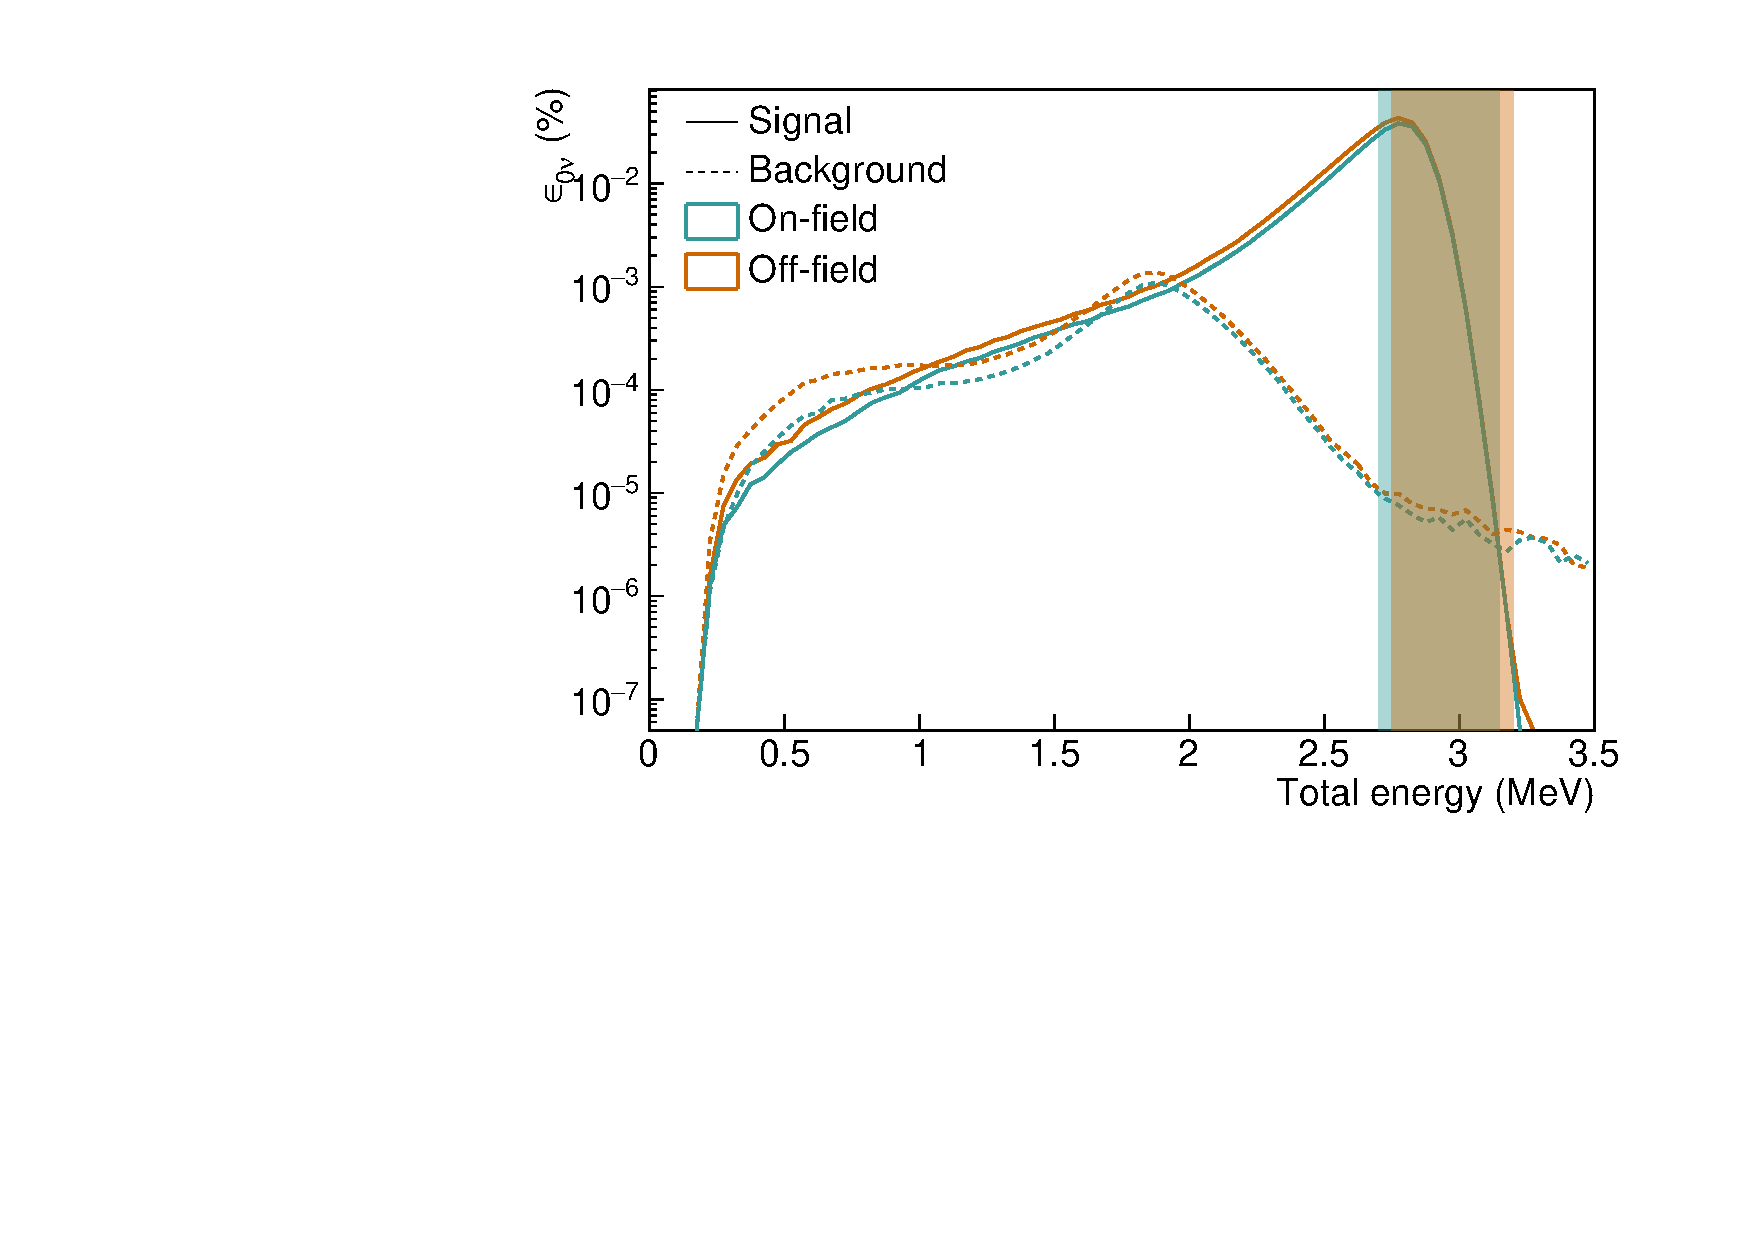
\includegraphics[width=0.8\textwidth]{Sensitivity/fig_sensitivity/Nbkg_field.pdf}
  \caption{The $\zeronu$ selection efficiency (plain line), and expected number of background events (dashed line), as a function of the $2e$ energy, for the on-field (blue) and the off-field (orange) cases.
    Results are presented for a $17.5$~kg.y exposure, for the specified isotope activities.
    The two corresponding region of interests are also displayed by coloured stripes.
    Here no optimised topological cut-offs have been applied.
    \label{fig:eff_0nu_w_wo_B}}
\end{figure}
The two coloured stripes represent the corresponding region of interests, of [$2.7$;$3.15$]~MeV for the \emph{on-field} case, and [$2.75$;$3.2$]~MeV for the \emph{off-field} case.
These results are presented for the specified contamination levels, but remain valid in all cases.
We clearly notice that, for the total energy interval [$0$;$4$]~MeV, the number of signal and background selected events is higher in the off-field case, which confirms what we were saying above.

Following Eq.~\eqref{eq:tbeta_limit}, the ratio $\epsilon_{0\nu}/N_{0\nu}^{\text{excl.}}$ in the ROI impacts the final sensitivity.
Nevertheless, as we explained in the previous section, the low contamination level considered causes $N_{0\nu}^{\text{excl.}}$ to reach the $2.303$ limit.
%the upper limit set on $\Tbeta$ depends on $\epsilon_{0\nu}$ as well as on $N_{0\nu}^{\text{excl.}}$, the number of signal events excluded.
Thus, only variations of $\epsilon_{0\nu}$ in the ROI, between on-field and off-field cases, are the source of modifications on the final sensitivity.
Integrating $\epsilon_{0\nu}$ over the ROI, we obtain $\epsilon_{0\nu}^{\text{on-field}}=0.15\%>\epsilon_{0\nu}^{\text{off-field}}=0.12\%$.
The selection efficiency for the on-field case is favoured by the lower bound of the ROI.
In fact, the further this lower bound is shifted towards lower energies, the greater the selection efficiency.
Besides, slight variations of the upper bound have almost no impact.
As expected, this results in a decrease in sensitivity when the field is switched off, giving
\begin{equation}
\Tbeta > 4.80\times 10^{24}\,\text{y}\qquad (90\% \text{CL})\, (\text{off-field}).
\end{equation}
We present in Tab.~\ref{tab:eff_field} the selection efficiencies of the signal and backgrounds, in the ROI, for the two field cases.
\begin{table}[h]
  \centering
  \begin{tabular}{|c|c|c|}
    \hline
    Process & On-field & Off-field \\
    \hline\hline
    $\epsilon_{0\nu}$ (\%) & $14.7$ & $12.4$ \\
    $\twonu$  & $0.40$ & $0.063$ \\
    \Tl  & $0.047$ & $0.060$ \\
    \Bi  & $0.054$ & $0.045$ \\
    \Rn  & $0.29$ & $0.55$ \\
    \hline
  \end{tabular}
  \caption{Expected number of background events in the $2e$ topology, in the ROI, for the SuperNEMO demonstrator (17.5 kg.y), for specified activities.
    The selection efficiency of $\zeronu$ events, $\epsilon_{0\nu}$, is also given.
    The two on- and off-field cases are compared.
    The region of interests are [$2.7$;$3.15$]~MeV for the on-field case, and [$2.75$;$3.2$]~MeV whan the field is switched-off.
    \label{tab:eff_field}}
\end{table}
We principally notice that the \Tl\ and \Rn\ contributions are higher in the second case.
As concluded in Sec.~\ref{sec:demonstrator_sensitivity}, topological selections are especially efficient in rejecting these two backgrounds.
Therefore, the application of these additionnal cut-offs, for the off-field case, could be interesting, in order to increase the sensitivity.
Following the work presented in the previous section, we optimise these selections for the particular off-field case, both for the specified and measured contamination levels\footnote{As done in sub-section~\ref{subsec:opti_ev_selection}, for the Bismuth measured contamination, we consider here the upper limit where $\mathcal{A}^{\text{Bi}}=290~\mu$Bq/kg.}.
The results in the sensitivity are summurised in Fig.~\ref{fig:sensitivity_B}.
\begin{figure}[h]
  \centering
  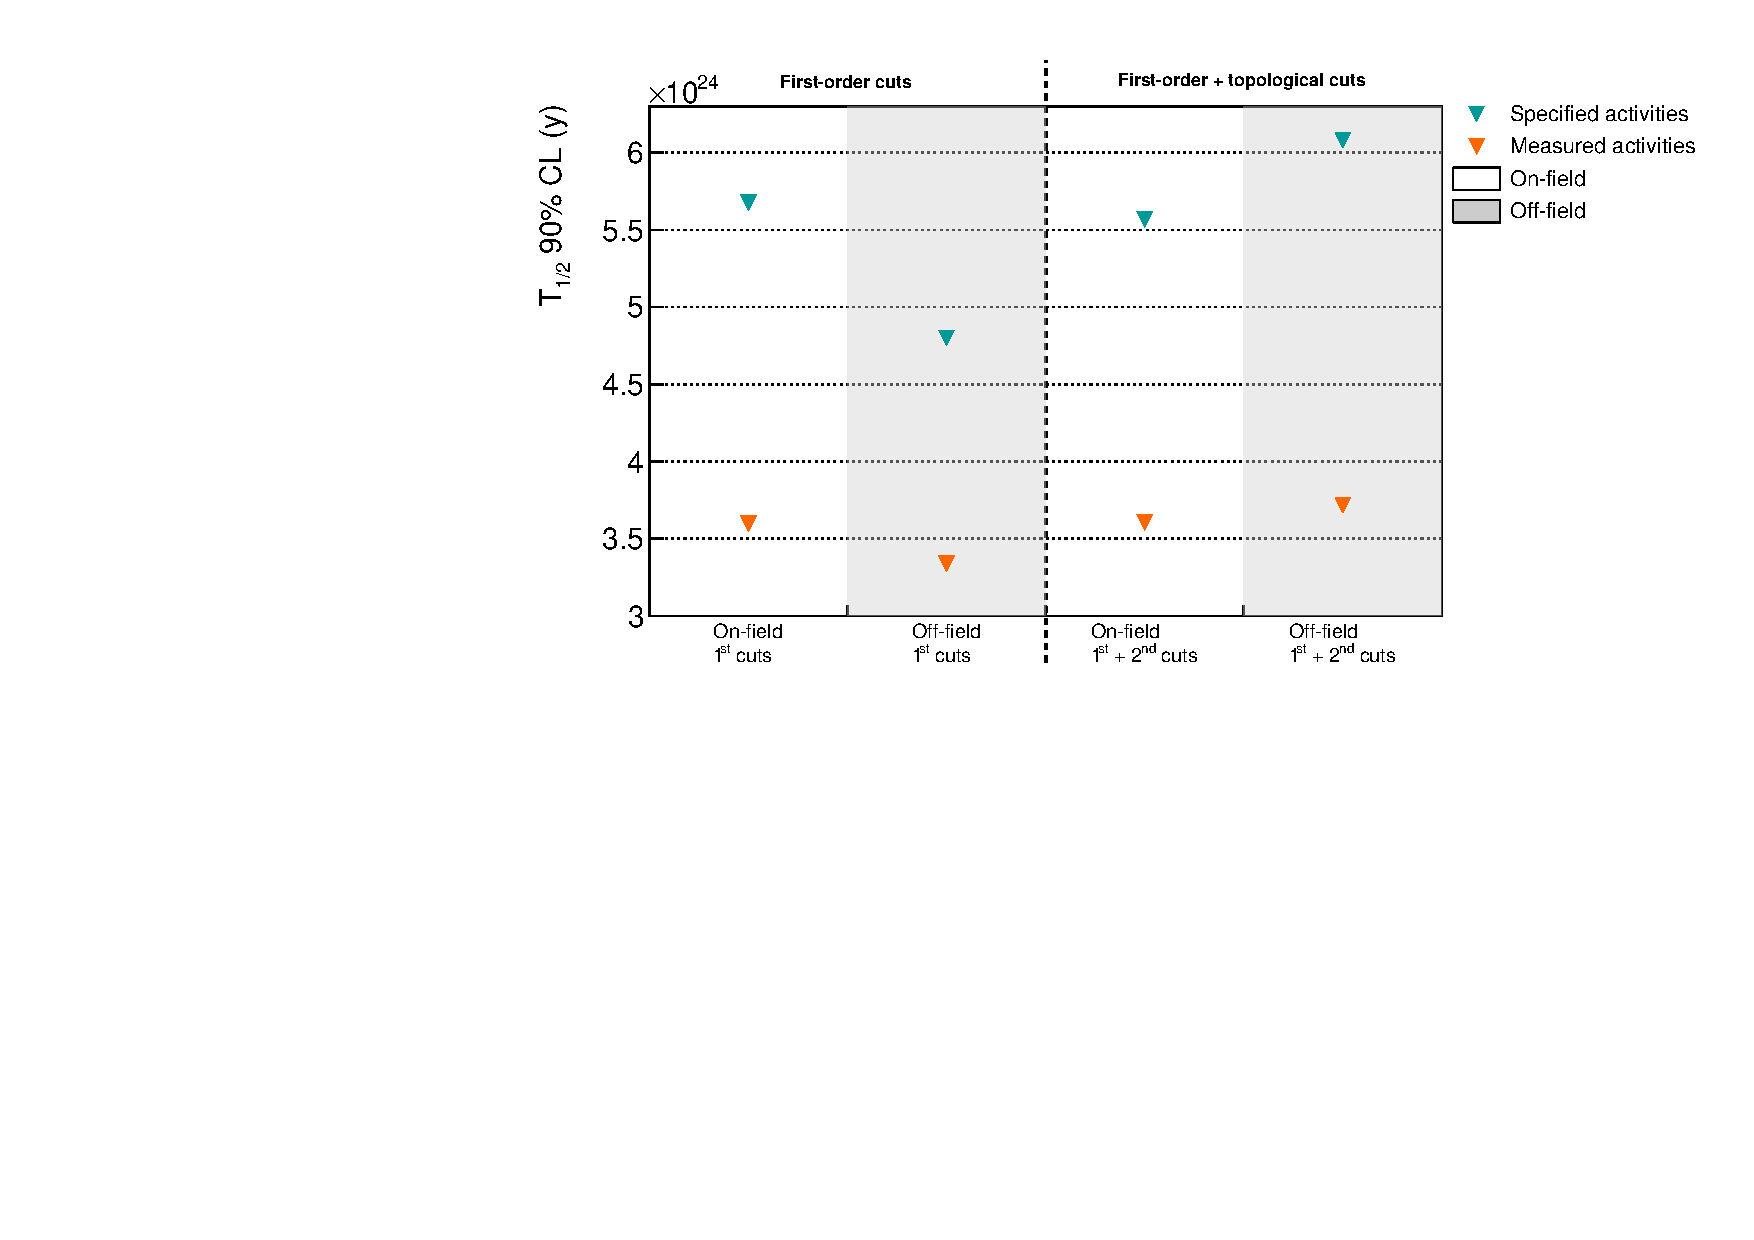
\includegraphics[width=1.1\textwidth]{Sensitivity/fig_sensitivity/contamination_Se_w_woB.pdf}
  \caption{$\Tbeta$ ($90$\% CL) considering various conditions: on- and off-field (white and gray stripes), first-order and addition of topological cut-offs (left/right parts of the panel), specified and measured activities (blue and orange triangle markers).
    The measured activities are $\mathcal{A}^{\text{Tl}}=54~\mu$Bq/kg, $\mathcal{A}^{\text{Bi}}=290~\mu$Bq/kg and $\mathcal{A}^{\text{Rn}} = 0.15$~mBq/m$^{3}$.
    \label{fig:sensitivity_B}}
\end{figure}
The left part of the panel gives information on the evolution of sensitivity, when only the first-order cut-offs are applied.
We come back to the conclusions given above: when the magnetic field is switched-off, we lose sensitivity, regardless of the level of contamination considered.
On the right side of the figure, we present the results when the topological cuts are applied.
For the on-field case, the addition of these selections have almost no effect on the sensitivity, as concluded in sub-section~\ref{subsec:opti_ev_selection}.
However, as predicted, we are beginning to see the usefulness of these selections in the off-field case, as a higher number of \Tl\ and \Rn\ events passed the first-order selections.
For instance, for the specification case, $\Tbeta$ goes from $4.80\times 10^{24}\,\text{y}$ to $6.1\times 10^{24}\,\text{y}$, an improvement of~$\sim~30\%$.

Finally, even if the absence of the magnetic field has the effect of reducing the sensitivity to the $\zeronu$ decay, topological cuts allow this effect to be compensated for, making it possible to reach higher values of $\Tbeta$.


%% \begin{itemize}
%% \item pour la variation de la ROI dans la figure comparative des différents level en contaminations : la ROI bouge pour les cas measured. C'est étonnant à premièer vue car ça ne paraît pas optimal et ça rajoute du Bi. Mais en fait si on regarde  les biplots de sensibilité, on a des fluctuations. Mais ce ne sont pas de grosses fluctuations, ce qui est aussi rassurant car ça veut dire qu'on n'est pas trop sensible aux variations de Emin/Emax (même si j'ai dit qu'on y était pas mal sensible -> à regarder)
%% \end{itemize}

\subsection{Influence of the magnetic field on optical modules and reconstruction efficiency}

In the previous sub-section, a comparative study has been lead to evaluate the influence of the presence of a magnetic field on the event selection, and thus on the final sensitivity.
However, as things stand now, some features of the demonstrator are not yet implemented in the simulations, and could have a great impact on the results presented above.
In particular, studies have been lead by the collaboration to evaluate the influence a $25$~Gauss magnetic field on the optical modules,  as well as on the event reconstruction~\cite{CalvezThesis}\cite{internal:magnetic_field}.

SuperNEMO PMTs are protected from the external magnetic field by individual, cylindrical, iron shields.
Unfortunately, the latter do not perfectly protect the PMTs, and a residual magnetic field is measured inside the shieldings, leading to charge losses close to $8\%$.
This study also revealed the energy resolution would be worsened, of $\sim 3\%$ of the initial value of $8\%$ at $1$~MeV.
Moreover, the PMTs shieldings could themselves severely impact the shape of the field lines, as well as its strength.
In fact, with a $25$ Gauss magnetic field generated by the copper coil, the magnetic shields are responsible for the field strength decreasing, and barely $10$ G is expected near the source foils.
Worse, the magnetic field strength decreases very quickly as we get closer to the calorimeter walls where nearly 0G could be expected.
The reconstruction efficiency could therefore be greatly impacted:
the magnetic field intensity varying from the source foils to the calorimeter wall, electrons trajectory curvatures are not constant, and the track-fitting algorithm is less performing.
And this effect is higher as the electron energy decreases.

In the light of these conclusions, it could be interesting to study the evolution of the sensitivity, considering field simulations with more realistic variations inside the detector.

%% Despite the fact that magnetic shields were designed and installed to protect the PMTs, this field can have a great impact on the calorimeter detection efficiency, and thus could degrade the detector's sensitivity to the $\zeronu$ decay.

\subsection{Simulations with a non-uniform magnetic field}
\label{subsec:mapped_field}

Simulations with a $25$ Gauss \emph{mapped} magnetic field have been performed, taking into account more realistic variations of the field inside the detector~\cite{docdb:map_magnetic_field2015}.
Unfortunately, not all isotopes could be simulated with this magnetic field configuration.
In particular, radon, as it is present in the entire wire chamber, would have required too many computing resources.
Thus, final conclusions on the sensitivity can't be given.
However, it is possible to assess the selection efficiencies of the different processes, and thus get an idea of the influence of realistic variations of the field on the final results.

%% Fig.~\ref{} displays
%% \begin{figure}[h]
%%   \centering
%%   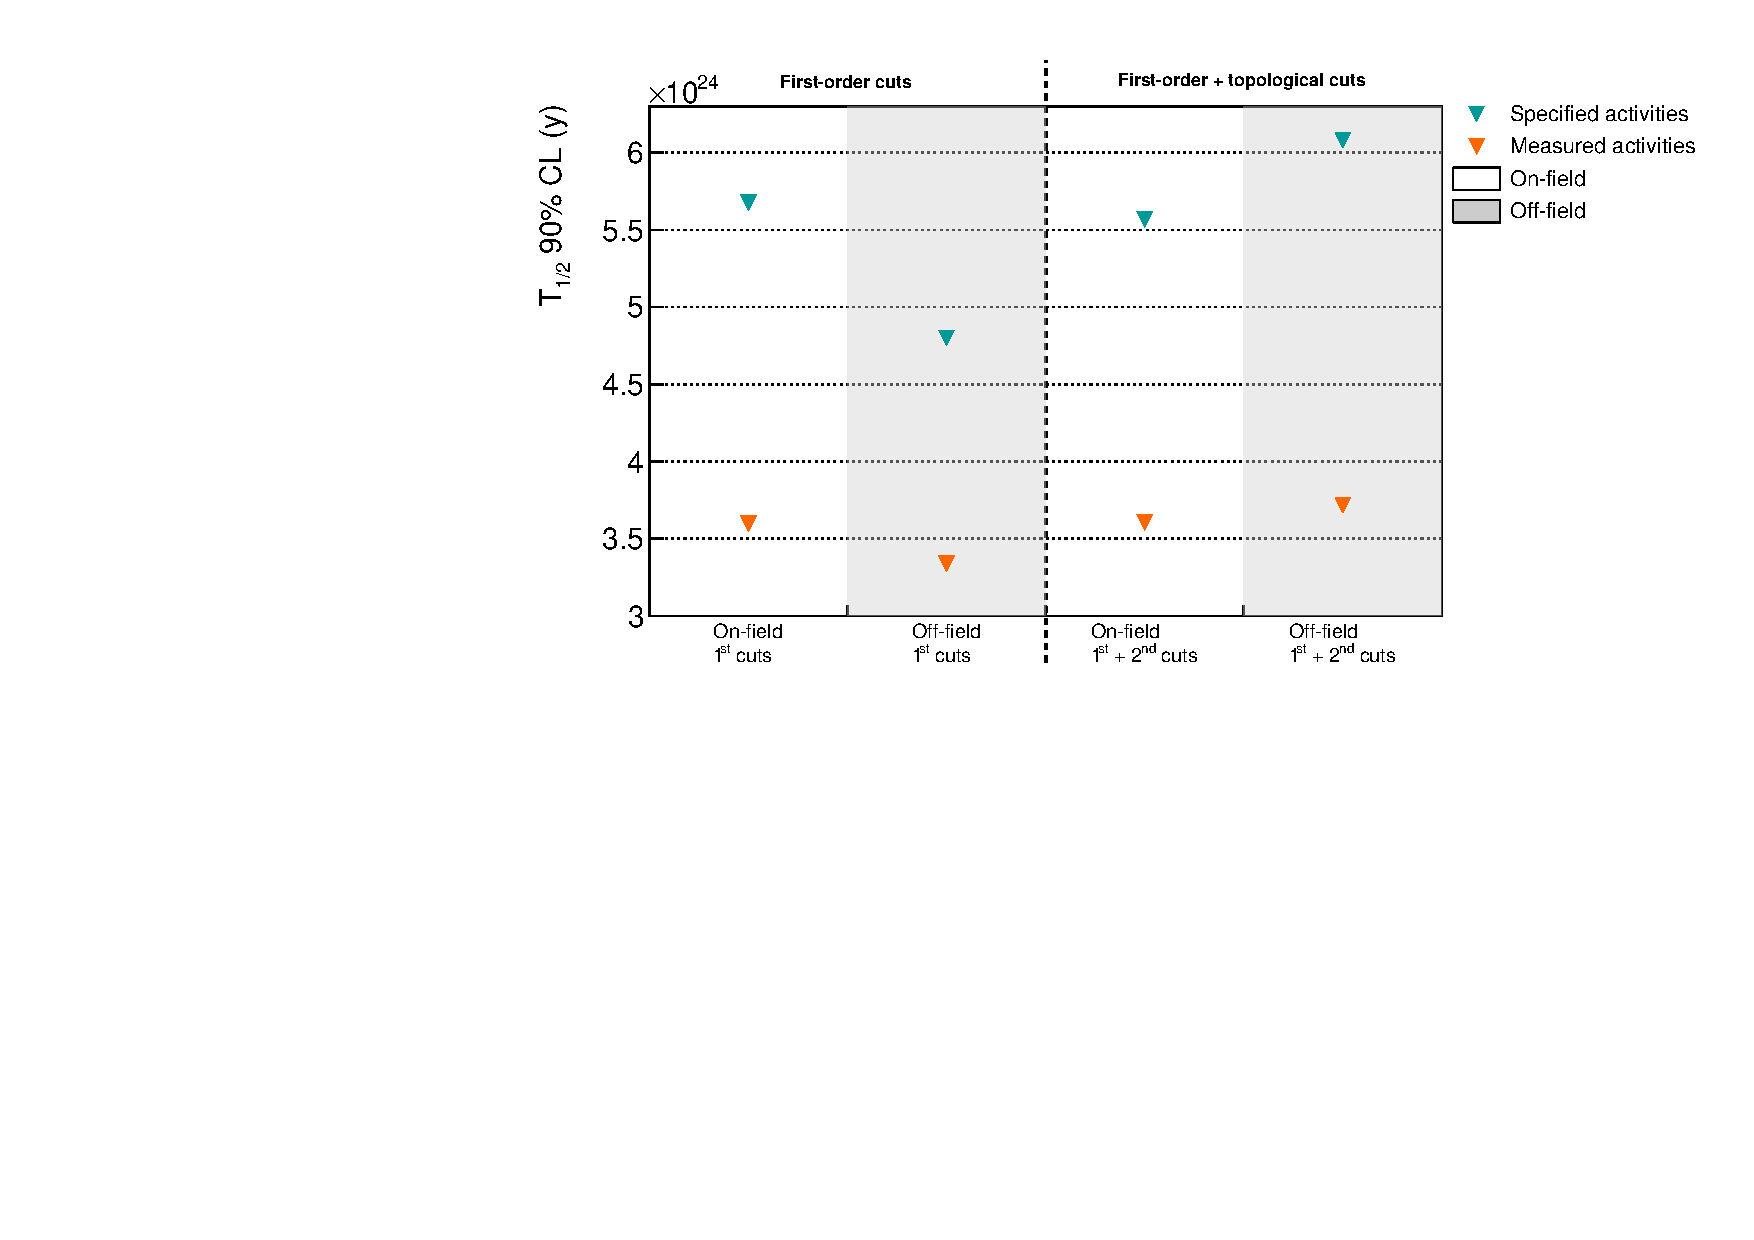
\includegraphics[width=1.1\textwidth]{Sensitivity/fig_sensitivity/contamination_Se_w_woB.pdf}
%%   \caption{Best limit set on $\zeronu$ half-life (top pad), and the corresponding ROI (bottom pad), as a function of the contamination level considered, for both on-field and off-field cases.
%%     \label{fig:}}
%% \end{figure}
Tab.~\ref{tab:mapped_eff} compares the selection efficiencies, for the three field cases (uniform field, mapped field and off-field), in the total energy range [$0$;$4$]~MeV.
\begin{table}[h]
  \centering
  \begin{tabular}{|c|ccc|}
    \hline
    & \multicolumn{3}{c|}{Selection efficiencies (\%)}\\
    Process & On-field & Off-field & Mapped-field  \\
    \hline\hline
    $\zeronu$ & $25.8$ & $29.7$ & $20.0$ \\
    $\twonu$ & $8.64$ & $9.93$ & $6.51$ \\
    \Tl & $0.0986$ & $0.152$ & $0.0910$ \\
    \Bi & $0.153$ & $0.220$ & $0.134$ \\
    \hline
  \end{tabular}
  \caption{Signal and background selection efficiencies of on-field, off-field and mapped-field cases, in the energy range [$0$;$4$]~MeV.
  \label{tab:mapped_eff}}
\end{table}
The mapped field case has lower selection efficiencies in the total energy range, compared with uniform field simulations.
As announced in the previous sub-section, the magnetic shields distort the field intensity accross the detector.
Therefore, the fitting algorithm is less performant in identifying particles with a negative curvature inside the tracker.


\begin{itemize}
\item du coup faudrait dire aussi que c'est la constatation de la variation de l'intensité du champ qui a motivé l'étude
\end{itemize}

\section{Searching for the Neodymium-$150~\zeronu$ decay}
\label{sec:Nd}

This study was conducted jointly with the PhD student Axel Pin, from CENBG~\cite{AxelThesis}.
Although we both worked on the whole of the analysis, I presented in detail, in the previous sections, the results regarding the influence of the magnetic field.
Meanwhile, Axel Pin present in detail the possibility of changing the Selenium material by other $\beta\beta$ isotopes.
Indeed, on the model of the NEMO-$3$ detector, which housed $6.914$~kg of \Mo\ and $0.932$~kg of \Se, the SuperNEMO detector has the technical possibility of exchanging the source material and study several $\beta\beta$ isotopes.
In the case SuperNEMO demonstrates the feasibility of a large-scale tracko-calo experiment, it would be natural to  evaluate the sensitivity of SuperNEMO to the $\zeronu$ decay of other isotopes than \Se.

\subsection{Searching for the $\zeronu$ of other isotopes}

As explained in Chapter~\ref{ch:detector}, the $2.615$~MeV $\gamma$-ray produced in the decay of \Tl\ is a troublesome source of background.
It is then important to select $\beta\beta$ candidates with a $\Qbb$ value above this transition.
The natural isotopic abundance is another useful criterion, and typically considering only isotopic abundances greater than 2\% is a good basis for making a choice.
Five nuclei satisfy these two criteria: $^{116}$Cd, \Se, \Mo, $^{96}$Zr and \Nd\ (with respective $\Qbb$ values of $2.80$, $2.99$,$3.03$, $3.35$ and $3.36$ keV and respective isotope abundance values of $7.5$, $9.2$, $9.6$, $2.8$ and $5.6$~\%~\cite{art:atomic_mass}).
Given the availability of \Mo, much effort has been focused by the NEMO-$3$ collaboration on this isotope (it had already been studied by the NEMO-$2$ prototype~\cite{art:NEMO2}).
As the \Nd\ isotope has the highest $\Qbb$ value, the current section focuses on evaluating the SuperNEMO sensitivity to the $\zeronu$ decay of this isotope, supposing we have several kg at our disposal.

\subsection{Sensitivity to the $\zeronu$ of \Nd}

Until recently, Neodymium was not enrichable in large quantities.
Recent developments have resulted in the production of several grams of enriched Neodymium, making this $\beta\beta$ isotope interesting for the search of $\zeronu$.
The best limit for the seach for neutrinoless double $\beta$ decay of \Nd\ was reached by the NEMO-$3$ detector, using $36.6$~g of enriched material for $5.25$~years of data acquisition.
The collaboration achieved $\Tbeta~<~2.0\times~10^{23}$~y~($90$~\%~CL), corresponding to an upper limit on the effective neutrino mass of $\langle\mbb\rangle~<~[1.6-5.3]$~eV.
The collaboration also measured the $\twonu$ half-life, with $\Ttwonu~=~$[$9.34~\pm~0.22$~(stat.)~+~$0.62-0.60$~(syst.)]$\times~10^{18}$~y~\cite{art:NEMO3_Nd}.

We wish to determine the limit on the $\zeronu$ of the \Nd\ that could be reached by the SuperNEMO demonstrator.
We lead this study considering the specified activities given for the \Se\ sources are reached.
We use simulations with the $25$~Gauss uniform magnetic field.
Fig.~\ref{fig:energy_Nd} presents the normalised energy distributions for the $2e$ topologies selected after application of first-order and topological selections.
\begin{figure}[h]
  \centering
  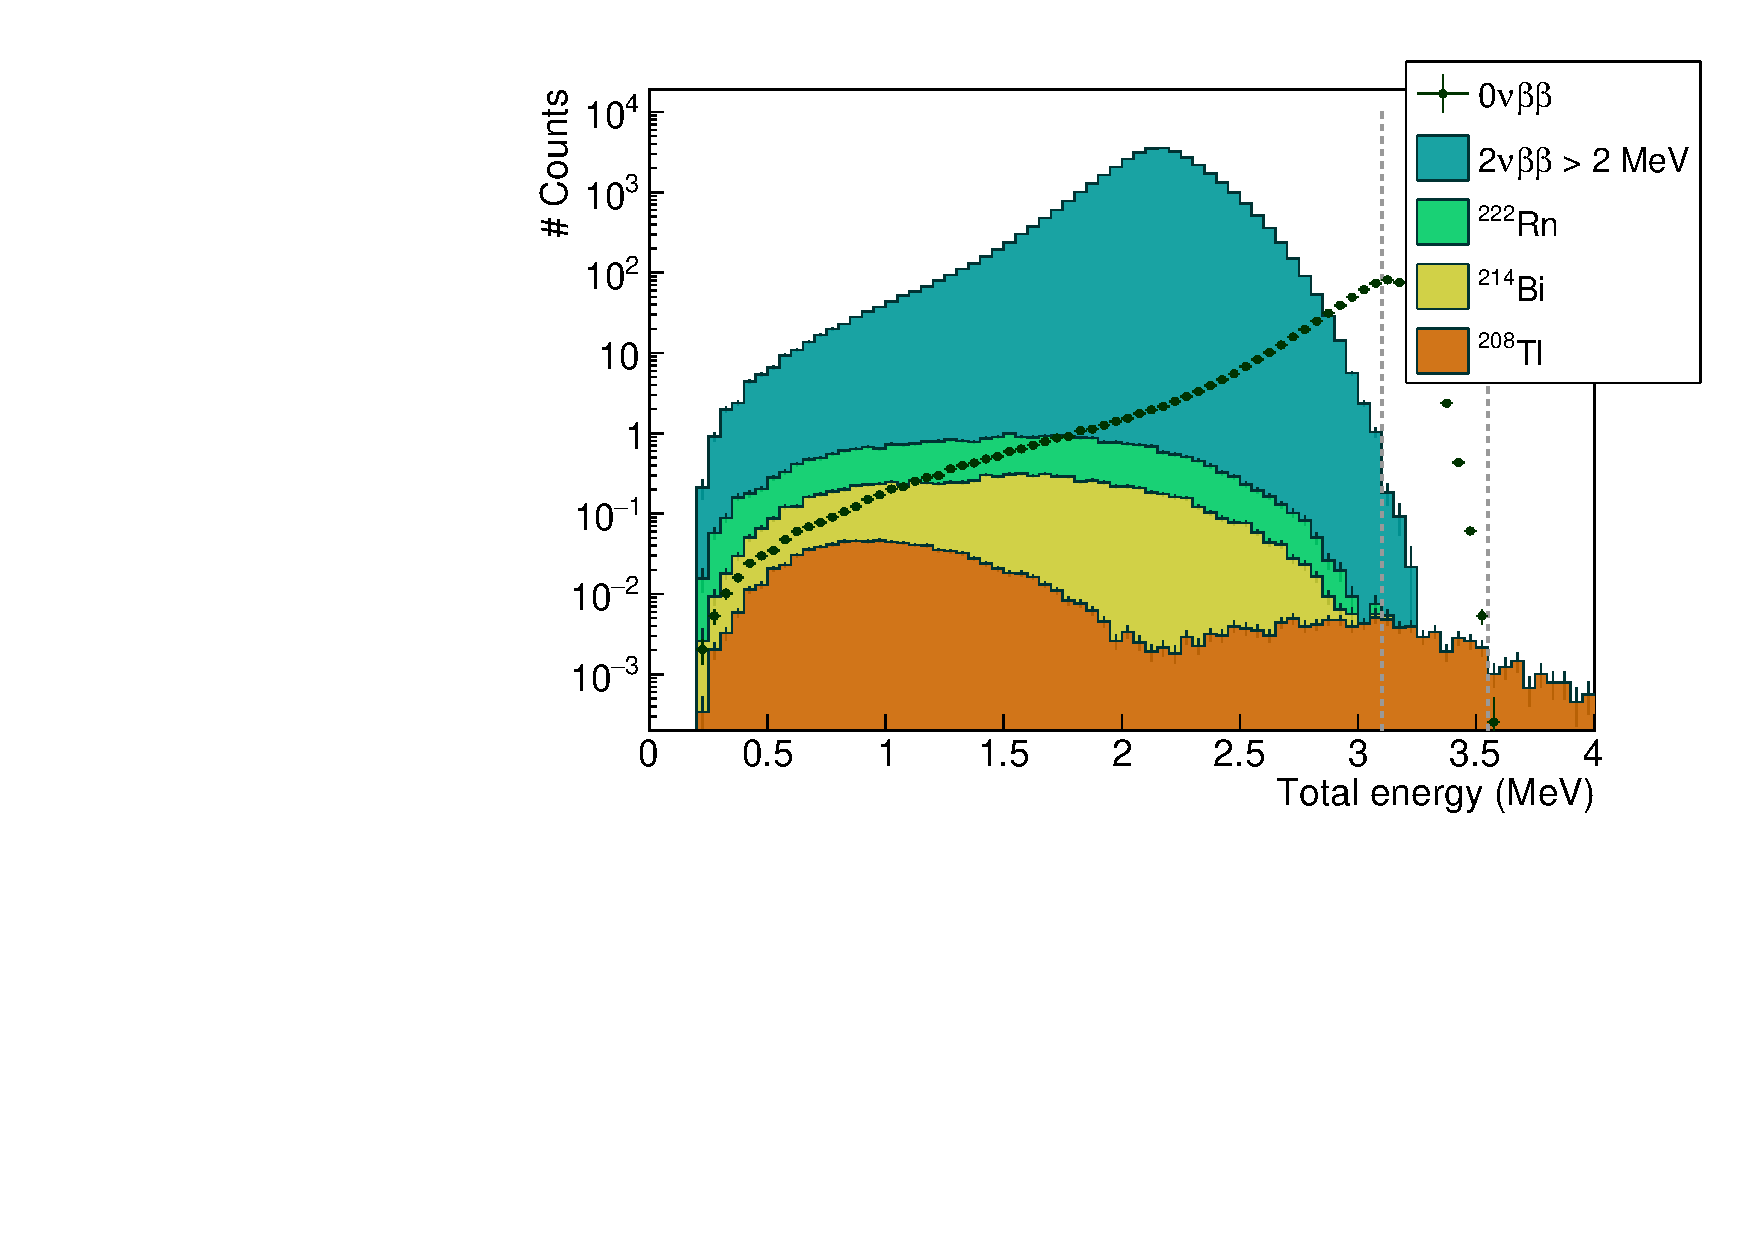
\includegraphics[width=0.8\textwidth]{Sensitivity/fig_sensitivity/energy_spectrum_with_B_150Nd.pdf}
  \caption{Normalised energy distributions of selected $2e$ topologies, for signal and background, in the case of \Nd\ sources.
    We assume a $17.5$~kg.y exposure.
    Specified activities are taken ($\mathcal{A}^{\text{Tl}} = 2~\mu$Bq/kg and $\mathcal{A}^{\text{Bi}} = 10~\mu$Bq/kg).
    First-order and optimised topological cuts have been applied.
    The $\beta\beta$ spectrum are normalised to $\Tbeta~=~2.0\times~10^{23}$~y ($90$~\% CL), and $\Ttwonu~=~9.34\times~10^{18}$~y~\cite{art:NEMO3_Nd}.
    The ROI of [$3.1$;$3.55$]~MeV is represented by to vertical dashed lines.
    \label{fig:energy_Nd}}
\end{figure}
Signal and background selection efficiencies for \Nd\ sources, in the total energy range, are given in Tab.~\ref{tab:energy_spect_Nd}.
\begin{table}[h]
  \centering
  \begin{tabular}{|c|cc|}
    \hline
    & \multicolumn{2}{c|}{Selection efficiencies (\%)} \\
    Process & Selenium & Neodynium \\
    \hline\hline
    $\zeronu$  & $25.8$ & $26.6$ \\
    $\twonu$  & $8.64$ & $8.85$ \\
    \Tl  & $0.0986$ & $0.0881$ \\
    \Bi  & $0.153$ & $0.147$ \\
    \Rn  & $0.0110$ & $0.0110$ \\
    \hline
  \end{tabular}
  \caption{Selection efficiencies in the full energy range [$0$;$4$]~MeV, after the application first-order and topological cut-offs.
    \label{tab:energy_spect_Nd}}
\end{table}
In this energy range, the background is dominated by the $\twonu$ decay.
The selection efficiencies of backgrounds are lower for \Nd\ sources than for \Se\ sources.
This is caused by the higher number of protons in the Neodynium nucleus.
Indeed, internal electrons are more likely to interact with the source material, by Coulombian interactions.
Then, in average, their energy is degraded, which increases their probability to undergone multiple scatterings inside the wire chamber, and then to be rejected by first-order cuts.
We used the same Radon simulations as for \Se\ sources, neglecting possible effects due to a higher proton number.

In Tab.~\ref{tab:eff_Nd_ROI} we give the expected number of background events in the ROI [$3.1$;$3.55$]~MeV.
\begin{table}[h]
  \centering
  \begin{tabular}{|c|c|c|}
    \hline
    Process & Selenium & Neodynium \\
    \hline\hline
    $\epsilon_{0\nu}$ (\%) & $14.4$ & $10.3$ \\
    $\twonu$  & $0.39$ & $0.28$ \\
    \Tl  & $0.044$ & $0.029$ \\
    \Bi  & $0.053$ & $5.6\times 10^{-4}$ \\
    \Rn  & $0.20$ & $0.0$ \\
    \hline
  \end{tabular}
  \caption{Expected number of background events in the ROI [$3.1$;$3.55$]~MeV, after the application first-order and topological selections.
    The demonstrator exposure of $17.5$~kg.y is considered, with specified activities.
    \label{tab:eff_Nd_ROI}}
\end{table}
The selection efficiency of the $\zeronu$ decay in this energy range is also given.
Although the $\twonu$ half-life of the \Nd\ is lower than that of the \Se\, the number of $\twonu$ events in the ROI remains low.
Indeed, thanks to the Coulombian effects described above, this process has a limited contribution at high energy.
The high energy of transition $\Qbb~=~3.36$~MeV of \Nd\ implies that the contributions of \Bi\ and \Rn\ are very small, or even zero.
The $\twonu$ and \Tl\ events are therefore the majority contributors to the background.

The SuperNEMO demonstrator, with $7$~kg of material and $2.5$~years of data acquisition, would achieve a $\Tbeta~>~2.2\times~10^{24}$~y sensitivity, one order of magnitude higher than the best limit ever reached.
The corresponding limit on the effective neutrino mass is $\langle\mbb\rangle~=~[0.15-0.50]$~eV.
This is a better result than for \Se\ sources, as the \Nd\ has a higher $G^{0\nu}$ factor.

%% The \Nd\ has a more favourable $\Qbb$ than \Se, with $\Qbb = 3.37$~MeV, .
%% However, its $\Ttwonu$ is lower, with $9.1\times 10^{18}$~years [ref].
%% For this study, we keep the \Se\ values for the contaminations, despite different purification efficiencies for the two isotopes.

\section{The final detector sensitivity}

The ultimate goal of the SuperNEMO demonstrator is to show that the NEMO technology is scalable to probe unprecedented half-life on the $\zeronu$ decay.
The final detector would consist in building $20$ modules similar to the demonstrator.

We suppose the specified activities of $\mathcal{A}^{\text{Tl}} = 2~\mu$Bq/kg, $\mathcal{A}^{\text{Bi}} = 10~\mu$Bq/kg and $\mathcal{A}^{\text{Rn}} = 0.15$ mBq/m$^{3}$ are reached.
The simulations with an uniform magnetic field are used.
With an exposure of $500$~kg.y, the SuperNEMO final detector should reach a sensitivity $\Tbeta~>~5.4\times~10^{25}$~y, with \Se\ sources.
The expected number of background events in the region of interest [$2.75$;$3.1$]~MeV being high enough, optimised topological cut-offs were applied, with \Pint\ $>~4~\%$ and $|\Delta~Z|~<80$~mm (samely for $|\Delta~Y|$).
The corresponding sensitivity to the neutrino mass is $\langle\mbb\rangle~=~[0.079-0.15]$~eV.


%% \begin{figure}[h]
%%   \centering
%%   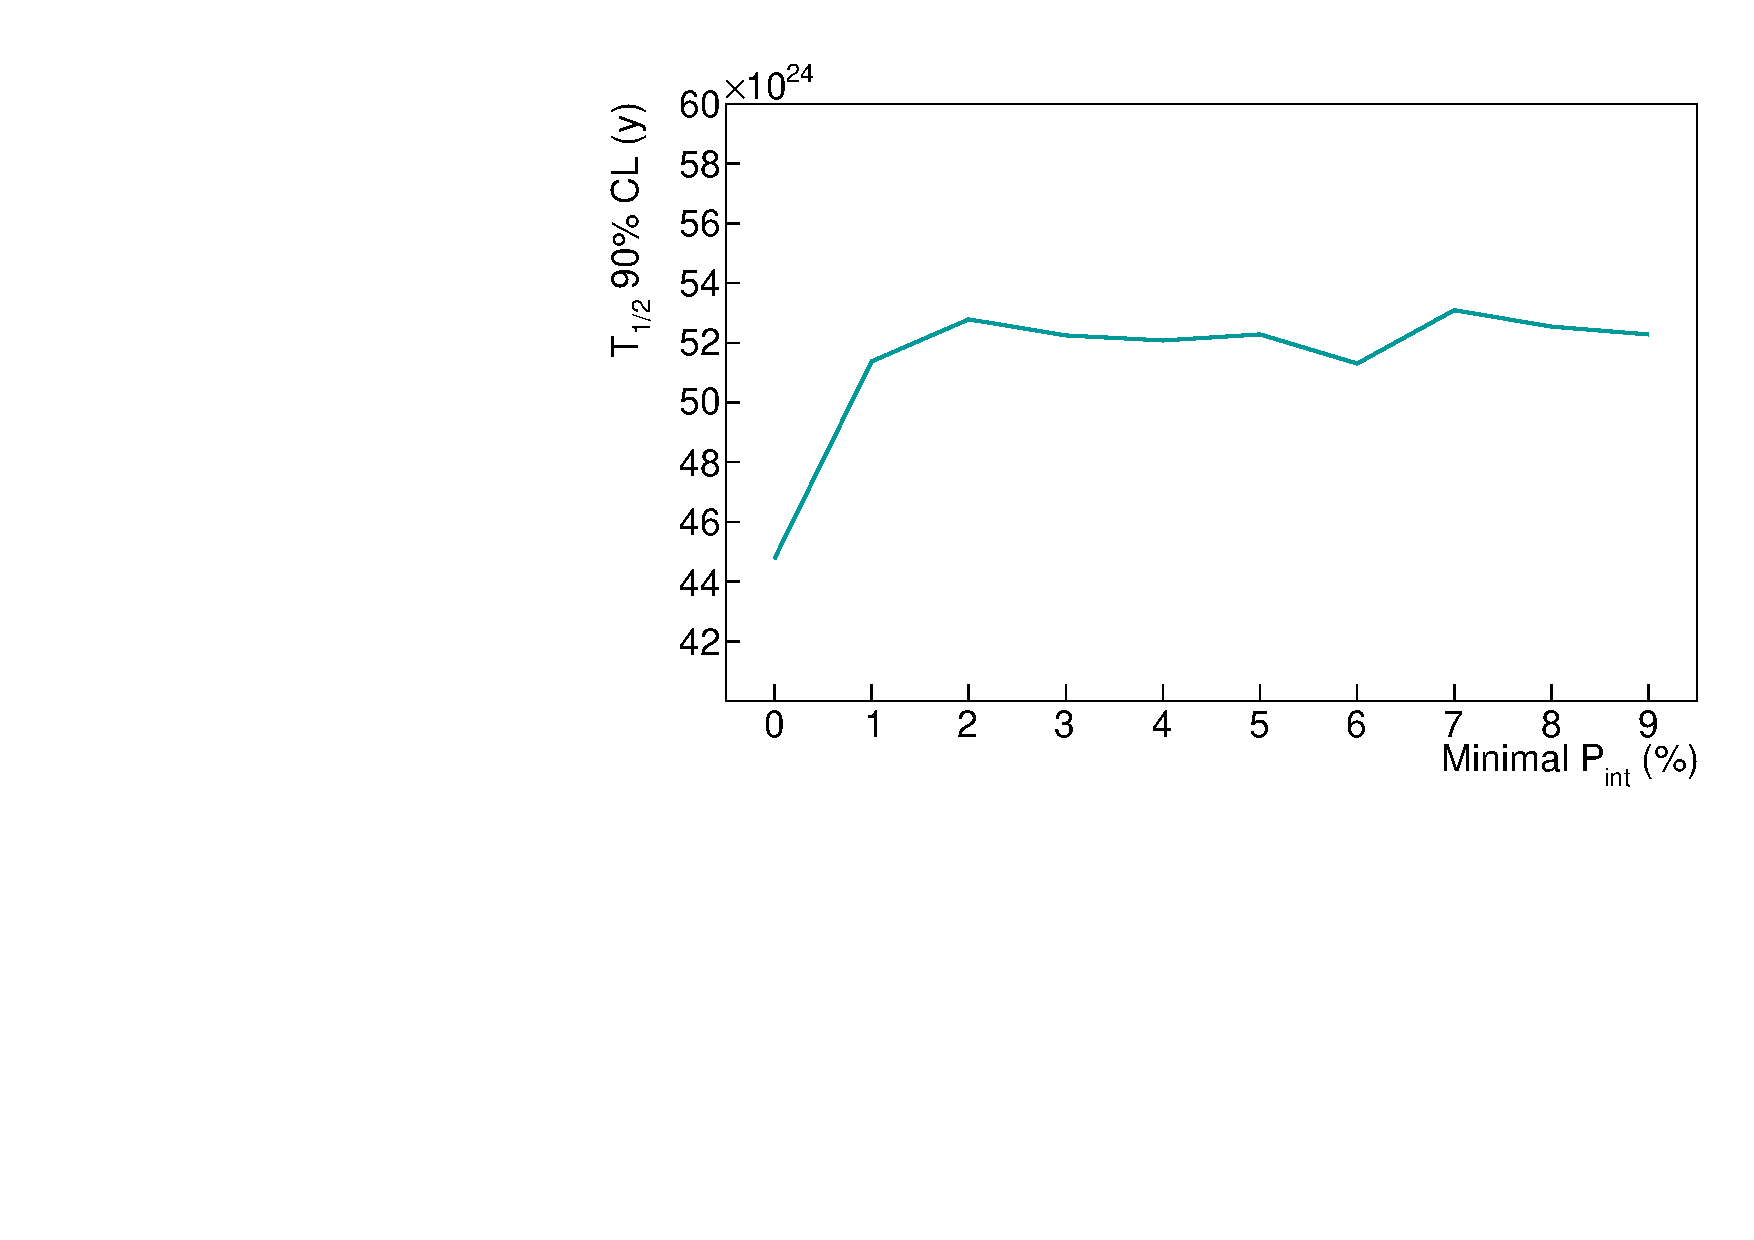
\includegraphics[width=0.8\textwidth]{Sensitivity/fig_sensitivity/HyperNEMO_T12_cut_Pint.pdf}
%%   \caption{
%%     \label{fig:HN_cut_Pint}}
%% \end{figure}




\section{Conclusion}

Assuming the target background levels are reached, the SuperNEMO demonstrator, running for two and half years with $7$~kg of \Se\ would be able to a set a limit on the $\zeronu$ process $\Tbeta~>~5.6\times~10^{24}$~years, translating into a limit on the neutrino effective mass $\langle\mbb\rangle~<~[0.25-0.48]$~eV (depending on the Nuclear Matrix Elements).
Latest measurements of source activities show that the specified background levels are not reached, although they were improved in average by a factor of 2, compared to NEMO-$3$.
To offset this, topological selections, designed to reject non-internal and non-simultaneous $2e$ events, have been optimised.
The calorimeter time resolution plays an important role on the cut-off efficiencies, especially on the internal probability.
Future studies would investigate the influence of this resolution on the final limit set on $Tbeta$.
Finally, assuming the worst activity is reached for the internal Bismuth isotope, we would set a limit on the $\Tbeta~>~3.6\times~10^{24}$~years, a decrease of $35$~\% compared to the specified activities result.
This corresponds to $\langle\mbb\rangle~<~[0.31-0.59]$~eV.
Finally, the limit on $\Tbeta$ could be enhanced by using a multivariate analysis, similarly to what is done in other double beta decay experiments, taking advantage of the several topological variables offered by SuperNEMO.

Recent studies have shown that the $25$~Gauss magnetic field would be distorted by detector materials, especially the calorimeter magnetic shields.
In this context, we studied the influence on the demonstrator sensitivity of the presence of magnetic field.
Switching-off the field would decrease the sensitivity, but can be compensated by the topological cut-offs, useful with such a level of background..
Finally, the absence of magnetic field would slightly increase the limit set on the sensitivity to $\Tbeta~>~3.7\times~10^{24}$~years, taking into account the measured activities, and $\langle\mbb\rangle~<~[0.30-0.58]$~eV.
Simulations with a mapped field shown that the signal and background selection efficiencies would be degraded by a non-uniform field.
A more complete study would also take into account the possible impacts on the calorimeter energy resolution.

Like its predecessor, the SuperNEMO demonstrator was designed to study several isotopes, such as the \Nd.
Assuming the target background activities are reached for \Nd\ sources, the SuperNEMO demonstrator would achieve a $\Tbeta~>~2.2\times~10^{24}$~years, and $\langle\mbb\rangle~<~[0.15-0.50]$~eV.

Finally, assuming we reach the target background levels, the superNEMO final detector would achieve an unprecedented limit of $\Tbeta~>~5.4\times~10^{25}$~years for \Se\ sources, and $\Tbeta~>~2.4\times~10^{25}$~years for \Nd\ sources.
To complete these results, the SuperNEMO collaboration would study the influence on the sensitivity of external backgrounds, coming from detector materials as well as the laboratory.


\begin{itemize}
\item Plot général récap tous résultats

\item manque de stat pour le neodyme car ROI haute E
\item légères diff avec résultats axel car légères diff dans sélections d'ev car utilisation PID

\item cellules tracker dead-> refaire analyse
\item delayed cells->improvement, cf NEMO 3
\end{itemize}
